%%%%%%%%%%%%%%%%%%%%%%%%%%%
% PREAMBOLO DEL DOCUMENTO %
%%%%%%%%%%%%%%%%%%%%%%%%%%%
\documentclass[a4paper,11pt,oneside,openright,reqno,table]{book}
% openany - fa iniziare i capitoli direttamente nella pagina successiva
% openright - fa iniziare i capitoli nella prima pagina destra disponibile 
% fleqn  - allinea le formule a sinistra anziché centrarle
% leqno - dispone la numerazione delle formule sulla sinistra o destra
% reqno - dispone la numerazione delle formule sulla destra
%
\usepackage{packages}
% Per non appesantire troppo questo file
% quasi tutti i pacchetti usati sono salvati in packages.sty
%

% Per avere la parola BOZZA scritta su tutte le pagine
\usepackage[italian,light,first,bottomafter]{draftcopy}
% funziona solo in modalità PS
% Invece per i PDF ho risolto così:
% pdftk tesi.pdf background bozza.pdf output tesi_bozza.pdf
%
\usepackage{float}
\usepackage{placeins}
\usepackage{setspace}   %Allows double spacing with the \doublespacing command
\usepackage{listings}
\usepackage{color}
\usepackage{interval}
\usepackage{gensymb}

\usepackage{booktabs, multirow} % for borders and merged ranges
\usepackage{soul}% for underlines
\usepackage[table]{xcolor} % for cell colors
\usepackage{changepage,threeparttable} % for wide tables

\usepackage{pdfpages}

\usepackage{siunitx}

\definecolor{tablelightgray}{gray}{0.9}
\definecolor{lightgray}{rgb}{0.95, 0.95, 0.95}
\definecolor{darkgray}{rgb}{0.4, 0.4, 0.4}
%\definecolor{purple}{rgb}{0.65, 0.12, 0.82}
\definecolor{editorGray}{rgb}{0.95, 0.95, 0.95}
\definecolor{editorOcher}{rgb}{1, 0.5, 0} % #FF7F00 -> rgb(239, 169, 0)
\definecolor{editorGreen}{rgb}{0, 0.5, 0} % #007C00 -> rgb(0, 124, 0)
\definecolor{orange}{rgb}{1,0.45,0.13}		
\definecolor{olive}{rgb}{0.17,0.59,0.20}
\definecolor{brown}{rgb}{0.69,0.31,0.31}
\definecolor{purple}{rgb}{0.38,0.18,0.81}
\definecolor{lightblue}{rgb}{0.1,0.57,0.7}
\definecolor{lightred}{rgb}{1,0.4,0.5}
\definecolor{mygreen}{RGB}{28,172,0} % color values Red, Green, Blue
\definecolor{mylilas}{RGB}{170,55,241}

\lstset{language=Matlab,%
    %basicstyle=\color{red},
    breaklines=true,%
    morekeywords={matlab2tikz},
    keywordstyle=\color{blue},%
    morekeywords=[2]{1}, keywordstyle=[2]{\color{black}},
    identifierstyle=\color{black},%
    stringstyle=\color{mylilas},
    commentstyle=\color{mygreen},%
    showstringspaces=false,%without this there will be a symbol in the places where there is a space
    numbers=left,%
    numberstyle={\tiny \color{black}},% size of the numbers
    numbersep=9pt, % this defines how far the numbers are from the text
    emph=[1]{for,end,break},emphstyle=[1]\color{red}, %some words to emphasise
    %emph=[2]{word1,word2}, emphstyle=[2]{style},    
}

\lstdefinelanguage{CSS}{
  keywords={color,background-image:,margin,padding,font,weight,display,position,top,left,right,bottom,list,style,border,size,white,space,min,width, transition:, transform:, transition-property, transition-duration, transition-timing-function},	
  sensitive=true,
  morecomment=[l]{//},
  morecomment=[s]{/*}{*/},
  morestring=[b]',
  morestring=[b]",
  alsoletter={:},
  alsodigit={-}
}
%configurazione codice php

% JavaScript
\lstdefinelanguage{JavaScript}{
  morekeywords={typeof, new, true, false, catch, function, return, null, catch, switch, var, if, in, while, do, else, case, break},
  morecomment=[s]{/*}{*/},
  morecomment=[l]//,
  morestring=[b]",
  morestring=[b]'
}

\lstdefinelanguage{HTML5}{
  language=html,
  sensitive=true,	
  alsoletter={<>=-},	
  morecomment=[s]{<!-}{-->},
  tag=[s],
  otherkeywords={
  % General
  >,
  % Standard tags
	<!DOCTYPE,
  </html, <html, <head, <title, </title, <style, </style, <link, </head, <meta, />,
	% body
	</body, <body,
	% Divs
	</div, <div, </div>, 
	% Paragraphs
	</p, <p, </p>,
	% scripts
	</script, <script,
  % More tags...
  <canvas, /canvas>, <svg, <rect, <animateTransform, </rect>, </svg>, <video, <source, <iframe, </iframe>, </video>, <image, </image>, <header, </header, <article, </article
  },
  ndkeywords={
  % General
  =,
  % HTML attributes
  charset=, src=, id=, width=, height=, style=, type=, rel=, href=,
  % SVG attributes
  fill=, attributeName=, begin=, dur=, from=, to=, poster=, controls=, x=, y=, repeatCount=, xlink:href=,
  % properties
  margin:, padding:, background-image:, border:, top:, left:, position:, width:, height:, margin-top:, margin-bottom:, font-size:, line-height:,
	% CSS3 properties
  transform:, -moz-transform:, -webkit-transform:,
  animation:, -webkit-animation:,
  transition:,  transition-duration:, transition-property:, transition-timing-function:,
  }
}

\lstdefinestyle{htmlcssjs} {%
  % General design
%  backgroundcolor=\color{editorGray},
  basicstyle={\footnotesize\ttfamily},   
  frame=b,
  % line-numbers
  xleftmargin={0.75cm},
  numbers=left,
  stepnumber=1,
  firstnumber=1,
  numberfirstline=true,	
  % Code design
  identifierstyle=\color{black},
  keywordstyle=\color{blue}\bfseries,
  ndkeywordstyle=\color{editorGreen}\bfseries,
  stringstyle=\color{editorOcher}\ttfamily,
  commentstyle=\color{brown}\ttfamily,
  % Code
  language=HTML5,
  alsolanguage=JavaScript,
  alsodigit={.:;},	
  tabsize=2,
  showtabs=false,
  showspaces=false,
  showstringspaces=false,
  extendedchars=true,
  breaklines=true,
  % German umlauts
  literate=%
  {Ö}{{\"O}}1
  {Ä}{{\"A}}1
  {Ü}{{\"U}}1
  {ß}{{\ss}}1
  {ü}{{\"u}}1
  {ä}{{\"a}}1
  {ö}{{\"o}}1
}
\lstdefinelanguage{Dockerfile}
{
  morekeywords={FROM, RUN, CMD, LABEL, MAINTAINER, EXPOSE, ENV, ADD, COPY,
    ENTRYPOINT, VOLUME, USER, WORKDIR, ARG, ONBUILD, STOPSIGNAL, HEALTHCHECK,
    SHELL},
  morecomment=[l]{\#},
  morestring=[b]"
}

\lstdefinestyle{lua}{
  language=[5.1]Lua,
  basicstyle=\ttfamily,
  keywordstyle=\color{magenta},
  stringstyle=\color{blue},
  commentstyle=\color{black!50}
  identifierstyle=\color{orange}
}


\usepackage[toc,page]{appendix}

 \renewcommand{\appendixname}{Appendice}
\renewcommand{\appendixpagename}{Appendici}

\usepackage[english]{babel}


%%%%%%%%%%%%%%%%%%%%%%%%%%%%%%%%%
%   DOCUMENTO VERO E PROPRIO    %
%%%%%%%%%%%%%%%%%%%%%%%%%%%%%%%%%
\begin{document}
% FRONTESPIZIO %
\begin{titlepage}
\changepage{}{}{}{-7.5 mm}{}{}{}{}{}

\newcommand{\HRule}{\rule{\linewidth}{0.5mm}}
\center
\begin{figure}[h]
	\centering
	
\includegraphics[scale=0.13]{frontmatter/figure/Unime.jpg}
\end{figure}
\textsc{\huge University of Messina}\\[0.5cm]
\textsc{\Large Department of Engineering}\\[0.3cm]
\textsc{\Large Engineering and Computer Science}\\[0.2cm]
\textsc{\Large Master's degree}\\[1.0cm]

\HRule\\[0.8 cm]

{ \huge \bfseries Robotic arm}\\[0.2cm]
{ \large Fischertecnick robotic arm }\\[0.5 cm]
\HRule \\[1.5 cm]

\begin{minipage}[t]{0.8\textwidth}
\begin{center}
{ \large Industrial automation and robotics mod.B}\\[0.3cm]
    
\end{center}
\end{minipage}

\vfill
\par
\noindent
\begin{minipage}[t]{0.47\textwidth}
	{\large{\textsc {Students:}} \\
		{\textbf{Gianluca Catalfamo}}\\
		{\textbf{Gabriele Morabito}}\\ 
		{\textbf{Giorgio Nocera}}\\
		{\textbf{Serena Sebbio}}\\
		} \\
\end{minipage}
\hfill
\begin{minipage}[t]{0.47\textwidth}\raggedleft
	{\large{\textsc{Teacher:}}} \\
		{\textbf{Prof. Eng. Luca Patanè}} \\
\end{minipage}
\vspace{15mm}


\begin{center}
    \HRule\\[0.5cm]
	{ACADEMIC YEAR 2020-2021}
\end{center}

\end{titlepage}

\doublespacing % interlinea 2
%

\frontmatter
% quello che segue è in numerazione romana e i capitoli non verranno numerati
% se non si vuole che compaia il numero di pagina basta usare il comando:
%\nonumber

% SOMMARIO %
%\include{frontmatter/sommario}
% INDICI %
\selectlanguage{english}
\phantomsection
\addcontentsline{toc}{chapter}{Index}
\tableofcontents
% Il simbolo * serve per evitare che comapaia nell'indice
\clearpage
%\listoffigures
%\clearpage
%\listoftables
% GLOSSARIO
%\cleardoublepage
\phantomsection
\addcontentsline{toc}{chapter}{Glossary}
% per inserire l'elenco dei simboli e degli acronimi nell'indice
\printglossary
% Per stampare il glossario
% per aggiornarlo si deve eseguire da terminale:
% makeindex -s myDoc.ist -t myDoc.alg -o myDoc.acr myDoc.acn
% per inserire una voce nell'elenco:
% \newglossaryentry{voce_etichetta}{name={voce}, description={descrizione}}
% se non compare direttamente nel testo va inizializzata con:
% \glsadd{voce_etichetta}
% oppure se viene richiamata all'interno del testo:
% \gls{voce_etichetta}
% SIMBOLI E NOTAZIONI %
%\cleardoublepage
\phantomsection
\addcontentsline{toc}{chapter}{List of Acronyms}
% per inserire l'elenco dei simboli e degli acronimi nell'indice
\printglossary[type=\acronymtype,title=List of Acronyms]
% Per stampare l'elenco dei simboli


nella figura \ref{6fig:iter} \\ 
\cite{8355223}
% per aggiornarlo si deve eseguire da terminale:
% makeindex -s myDoc.ist -t myDoc.glg -o myDoc.gls myDoc.glo
% per inserire una voce nell'elenco:
% \newglossaryentry{voce_etichetta}{name={voce}, description={descrizione}}
% se non compare direttamente nel testo va inizializzata con:
% \glsadd{voce_etichetta}
% oppure se viene richiamata all'interno del testo:
% \gls{voce_etichetta}

\mainmatter
% quello che segue sarà in numerazione araba e i capitoli verranno numerati
%\part{Studio iniziale}
% CAPITOLI
\chapter{Introduction} \label{1cap:introduction}
As part of the final exam of Industrial Automation and Robotics - part B, a Fischertechnick robotic arm has been controlled by a Siemens SIMATIC S7-1200 PLC through Siemens Totally Integrated Automation (TIA) Portal software environment. %and MATLAB.

% cosa fa ad alto livello: 
% 3 buttons: activate connection, reset, stop,
%controllo da remoto con matlab:
% rotation 0-3300
% horizontal 0-78
% vertical 0-1800
%gripper open/close

% green led and red led  s

\section{Goal of the project}
The goals of this project are:
\begin{itemize}
    \item to manage to implement an high level control system of a robotic arm using MATLAB, TIA Portal and a Siemens SIMATIC S7-1200 PLC;
    \item to create a 3D model of the robot, to simulate its behaviour and to compute the direct and inverse kinematic;
    \item to validate the model performing a simple task in the real world: pick up an object, move it to another position and release it.
\end{itemize}
\chapter{Enabling technologies} \label{2cap:design}
%
%\label{}

\section{Hardware}

\subsection{PLC SIMATIC S7-1200}
The PLC SIMATIC S7-1200 with CPU 1215C AC/DC/RLY (Figure\ref{fig:plc}) is a PLC produced by Siemens and it was used in this project in order to realize the sequence control of the robotic arm. \newline
It is characterized by:
\begin{itemize}
    \item 14 24V digital inputs;
    \item 10 relay outputs;
    \item 2 analog inputs;
    \item 2 analog outputs.
\end{itemize} 

\begin{figure}[!h]
\begin{center}
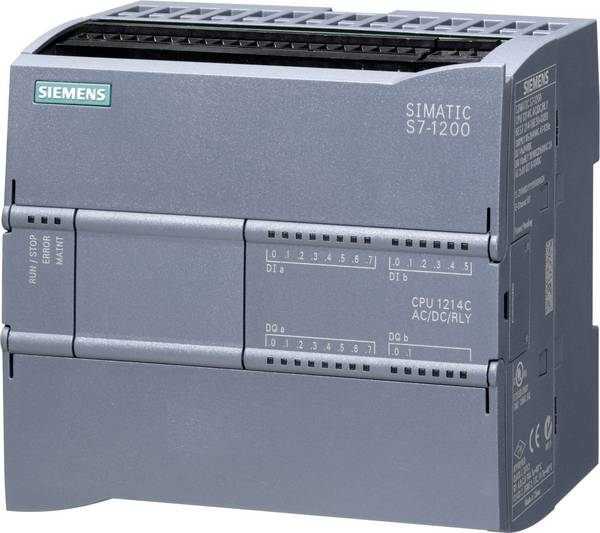
\includegraphics[width=0.4\linewidth]{capitolo2/figure/plc.jpeg}
\caption{Siemens SIMATIC S7-1200 1215C AC/DC/RLY PLC}
\label{fig:plc}
\end{center}
\end{figure}

\subsection{Fischertechnik 3D-Robot 24V}

The 3D-Robot 24V (Figure\ref{fig:robot}) is a robotic arm produced by Fischertechnik. It is a 3-DOF (3 degrees of freedom) robot and in particular it is composed by:
\begin{itemize}
    \item a revolute joint;
    \item 2 prismatic joints (up/down and frontward/backward);
    \item a gripper as end-effector.
\end{itemize}

\begin{figure}[!h]
\begin{center}
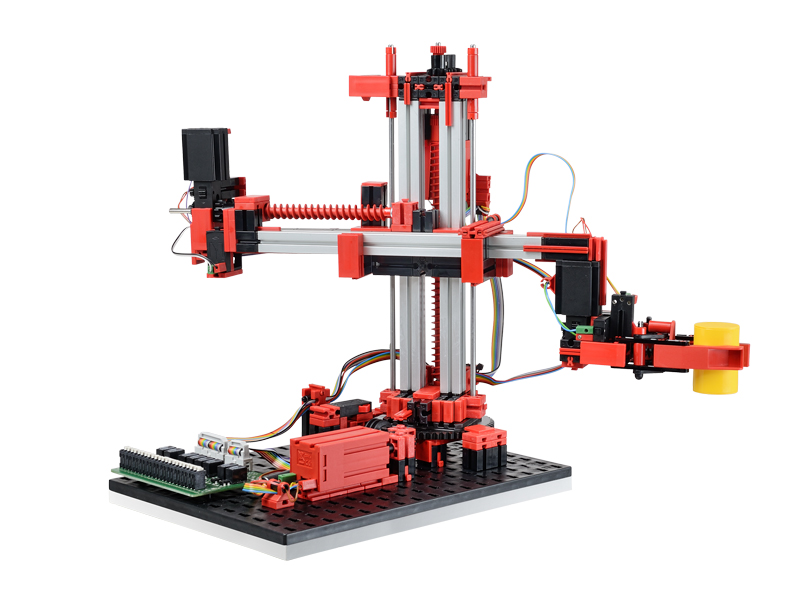
\includegraphics[width=0.8\linewidth]{capitolo2/figure/3D-Robot-24V.jpeg}
\caption{Fischertechnik 3D-Robot 24V}
\label{fig:robot}
\end{center}
\end{figure}
Thus the robot is characterized by a cylindrical geometry: its workspace is a portion of a hollow cylinder.

\subsubsection{Mini switches}
The robot has four mini switches (Figure\ref{fig:switch}) that are pressed respectively in four different conditions:
\begin{itemize}
    \item the gripper is fully open;
    \item the end-effector is completely brought back;
    \item the horizontal arm is completely brought up;
    \item the robot is completely rotated clockwise.
\end{itemize}

\begin{figure}[!h]
\begin{center}
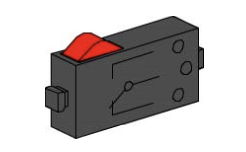
\includegraphics[width=0.4\linewidth]{capitolo2/figure/mini_switch.png}
\caption{Mini switch}
\label{fig:switch}
\end{center}
\end{figure}

\subsubsection{Pulse counters}
The robot has two pulse counters, that can be used to understand respectively:
\begin{itemize}
    \item how much the gripper is open;
    \item how much the horizontal arm is moved frontward.
\end{itemize}

In fact, the pulse counters are switches that are automatically pressed each time a gear involved in the corresponding movement rotate of a certain angle, producing a certain quantity of movement.

\subsubsection{Encoders}
The robot has two motor encoders (Figure\ref{fig:encoder}) with a maximum frequency of 1 KHz, that can be used to understand respectively:
\begin{itemize}
    \item how much end horizontal arm is moved down;
    \item how much the robot is rotated.
\end{itemize}

\begin{figure}[!h]
\begin{center}
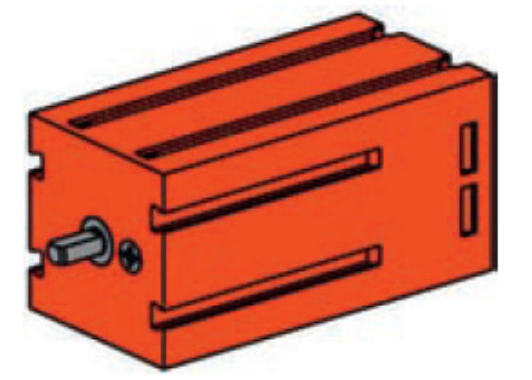
\includegraphics[width=0.4\linewidth]{capitolo2/figure/encoder.png}
\caption{Motor encoder}
\label{fig:encoder}
\end{center}
\end{figure}

\begin{figure}[!h]
\begin{center}
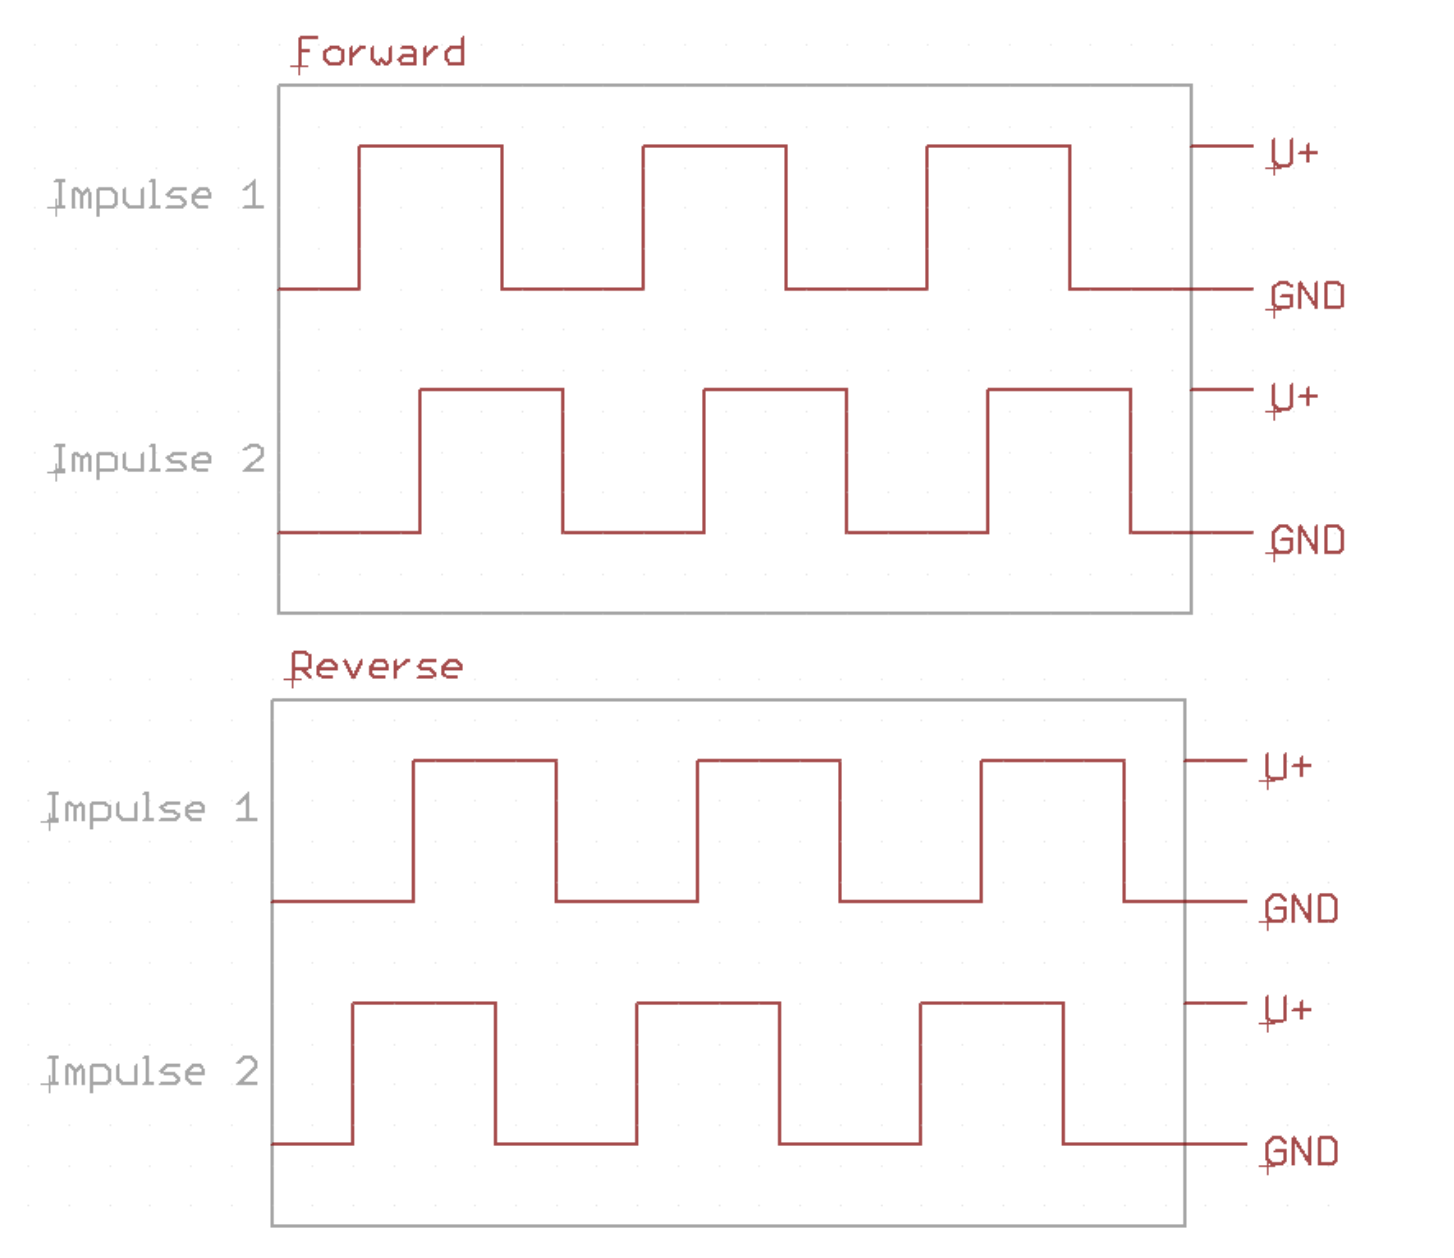
\includegraphics[width=0.8\linewidth]{capitolo2/figure/encoder_signals.png}
\caption{Encoder signals}
\label{fig:encoder_signals}
\end{center}
\end{figure}

The direction of the movement/rotation can be understood by the time order of the two signals generated by the encoder (Figure\ref{fig:encoder_signals}).

\subsection{Push-buttons}
In this project, three LM2T metal push-buttons with spring return produced by Lovato Electronics are used:
\begin{itemize}
    \item a black one (8 LM2T B102) with a normally open contact element is used for the reset operation that moves the robot to the initial position;
    \item a black one (8 LM2T B102) with a normally open contact element is used to start the TCP connection between the PLC and MATLAB;
    \item a red one (8 LM2T B104) with a normally closed contact element is used as a stop emergency button to stop the robot immediately.
\end{itemize}
\begin{figure*}[!h]
\centering
\subfloat[Push-button\label{fig:pushbutton}]{
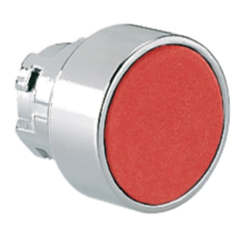
\includegraphics[width=0.25\linewidth]{capitolo2/figure/Push_button.png}
}
\qquad
\subfloat[Normally open contact element\label{fig:no}]{
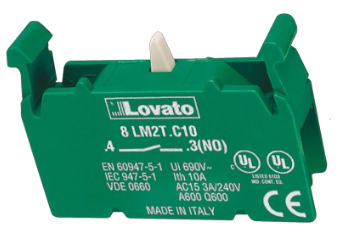
\includegraphics[width=0.25\linewidth]{capitolo2/figure/Normal_open.png}
}
\qquad
\subfloat[Normally closed contact element\label{fig:nc}]{
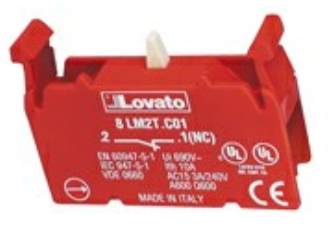
\includegraphics[width=0.25\linewidth]{capitolo2/figure/Normal_closed.png}
}
\caption{Push-buttons}
\label{fig:pushbuttons}
\end{figure*}

\subsection{Light Emitting Diodes}
Two Light Emitting Diodes produced by Lovato Electronics are used in this project. Each LED is made of a LED integrated lamp-holder, a mounting adapter and a pilot light head.
A green LED is turned on when the robot is ready to move and it blinks while the robot is moving.
A red LED is turned on after the emergency stop button has been pressed and it blinks during the reset operation.
\begin{figure*}[!h]
\centering
\subfloat[Light integrated lamp-holder\label{fig:led_integrated}]{
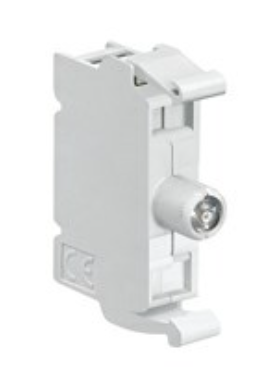
\includegraphics[width=0.25\linewidth]{capitolo2/figure/LED.png}
}
\qquad
\subfloat[Mounting adapter\label{fig:mounting_adapter}]{
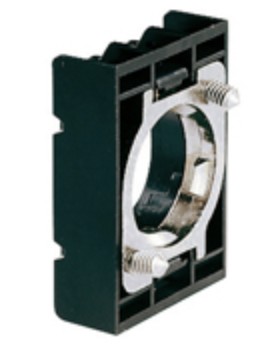
\includegraphics[width=0.25\linewidth]{capitolo2/figure/Mounting_adapter.png}
}
\qquad
\subfloat[Pilot light head\label{fig:light_head}]{
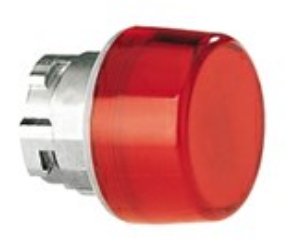
\includegraphics[width=0.25\linewidth]{capitolo2/figure/Light_head.png}
}
\caption{LED}
\label{fig:led}
\end{figure*}

\section{Software}

\subsection{TIA Portal}
TIA Portal (Totally Integrated Automation Portal) is a software package by Siemens created specifically to develop automation using Siemens products such as PLCs. It is in practice a centralized design environment characterized by a common user interface for all automation tasks with shared services (such as those of configuration, communication and diagnostics) and a single database to which also other software packages, such as SIMATIC WinCC V12, SINAMICS Startdrive V12 and SIMATIC STEP 7 PLCSIM V12, access.
The version 15 of the software was used in this project in order to design and upload the control program in the PLC.
TIA Portal has a user interface characterized by the presence of two views:
\begin{itemize}
    \item the portal view;
    \item the project view.
\end{itemize}

\begin{figure*}[!h]
\centering
\subfloat[Portal view\label{fig:portal_view}]{
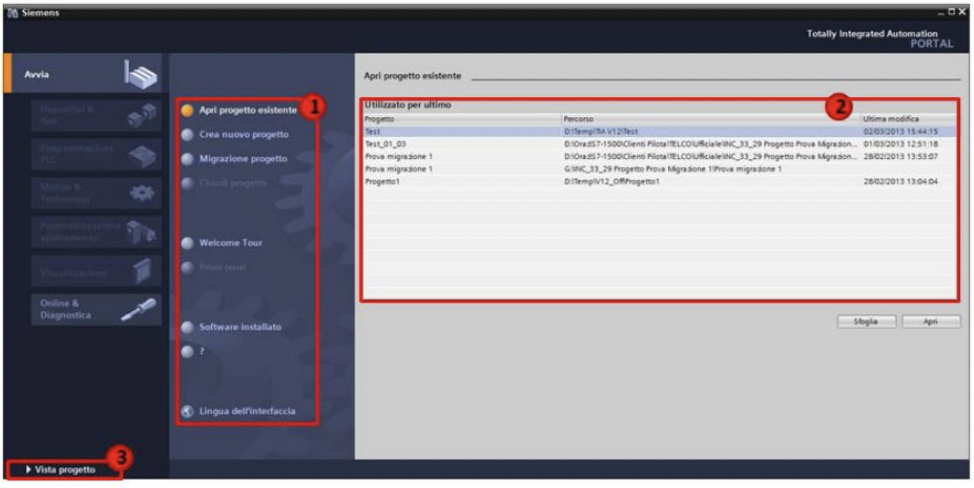
\includegraphics[width=0.45\linewidth]{capitolo2/figure/portal_view.png}
}
\qquad
\subfloat[Project view\label{fig:project_view}]{
\includegraphics[width=0.45\linewidth]{capitolo2/figure/project_view.png}
}
\caption{TIA Portal}
\label{first_signal}
\end{figure*}

\subsubsection{Portal view}
The portal view is the one that opens automatically when it is launched the TIA Portal and that allows the user to choose which operations he wants to perform with the TIA Portal. It is characterized by the presence of:
\begin{enumerate}
    \item a window where it is possible to choose which operation you want to perform;
    \item a selection window related to the selected operation;
    \item a button that allows to switch to the project view.
\end{enumerate}

\subsubsection{Project view}
The project view is the working window of the TIA portal that allows the performance of any function within a project; from the project view it is possible to access all the components of the project and quickly navigate within it.
It is characterized by the presence of:
\begin{enumerate}
    \item a window where it is possible to access and navigate all the components of the project;
    \item a window where the content of the component selected in window 1 is visualized;
    \item a window that allows the user to make changes to the project: the editors for writing of the software, the definition of the hardware or the definition of the panel pages based on the context in which the user is located are displayed;
    \item a window where it is possible to view the properties and the details of the objects selected in the window 3;
    \item a window that varies according to the editor that comes presented in window 3 and allows to view and use the TIA Portal Libraries tool.
\end{enumerate}


%\begin{figure}[!h]
%\begin{center}
%\includegraphics[width=0.8\linewidth]{figure/project_view.png}
%\caption{TIA Portal project view}
%\end{center}
%\label{fig:layout}
%\end{figure}  



%
%\begin{figure*}[!h]
%\centering
%\subfloat[First input signal\label{fig:first}]{%
%\includegraphics[width=0.45\linewidth]{capitolo2/figure/firstinp%ut_out.PNG}%
%}
%\qquad
%\subfloat[First input signal outlier\label{fig:first_det}]{%
%\includegraphics[width=0.45\linewidth]{capitolo2/figure/firstinp%ut_out_detail.PNG}%
%}
%\caption{Plot of the first input signal}
%\label{first_signal}
%\end{figure*}

\subsection{MATLAB}
MATLAB (an abbreviation of "matrix laboratory") is a programming and numeric computing platform developed by MathWorks. MATLAB allows matrix manipulations, plotting of functions and data, implementation of algorithms, data analysis, creation of user interfaces, and interfacing with programs written in other languages.
After starting MATLAB, the desktop appears in its default layout.
\begin{figure}[!h]
\begin{center}
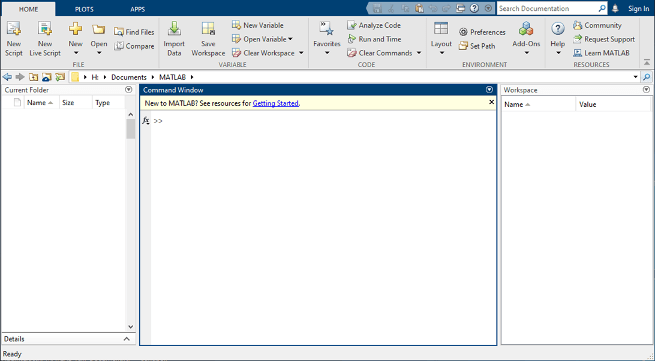
\includegraphics[width=0.6\linewidth]{capitolo2/figure/matlab_desktop.png}
\caption{Matlab desktop}
\end{center}
\label{fig:matlab_desktop}
\end{figure}


The desktop includes these panels:
\begin{itemize}
    \item Current Folder — for file access
    \item Command Window — for entering commands at the command line, indicated by the prompt (>>)
    \item Workspace — for exploring data created or imported from files. \cite{MATLABDo23:online}
\end{itemize} 
%source: matlab documentation
%verify version
In this project a TCP communication between MATLAB (R2021a) and TIA Portal is established to send and receive data continuously. 

\subsection{CoppeliaSim}
CoppeliaSim, formerly known as V-REP (Virtual Robot Experimentation Platform), is a general purpose robot simulator, with integrated development environment, used in industry, education and research for fast algorithm development, factory automation simulations, fast prototyping and verification, robotics related education, motion planning, remote monitoring and safety double-checking. 
CoppeliaSim is based on a distributed control architecture: each object/model can be individually controlled via an embedded script, a plugin, a ROS or BlueZero node, a remote API client, or a custom solution. This makes CoppeliaSim very versatile and ideal for multi-robot applications. Controllers can be written in C/C++ (plug-ins), Lua (scripts acting as individual synchronous controllers), Python, Java,  Matlab or Octave (asynchronous controllers). \cite{Robotsim90:online}
% reference: https://www.coppeliarobotics.com/
% wikipedia:
At its core, CoppeliaSim uses a kinematics engine for forward and inverse kinematics calculations, and several physics simulation libraries to perform rigid body simulation. Models and scenes are built by assembling various objects (meshes, joints, various sensors, Point clouds, OC trees, etc.) into a hierarchial structure. Additional functionality, provided by plug-ins, include: motion planning (via OMPL), synthetic vision and imaging processing (e.g. via OpenCV), collision detection, minimum distance calculation, custom graphical user interfaces and Data visualization (e.g. via plots). \cite{Coppelia94:online}


Scene objects are basic building blocks that can be combined with each other. They can form complex systems together with calculation modules and control mechanisms.

There are fourteen types of scene objects: proximity sensors, graphs, vision sensors, paths, mills, cameras, lights, mirrors, shapes, joints, force / torque sensors, dummies, octrees and point clouds.

There are five calculation modules:
\begin{itemize}
    \item Collision detection
    \item Physics / Dynamics
    \item Minimum distance calculation
    \item Path / Motion planning
    \item Forward / Inverse kinematics
\end{itemize}
%Control mechanisms
%6 methods or interfaces
%>7 languages
%6 methods can be used at the same
%time, and even work hand in hand




 

\chapter{Implementation}

\section{Analisys}
To analyze the behaviour of the robot, a first step is related to its kinematic. Kinematic analysis of the mechanical structure of a robot concerns the description of the motion with respect to a fixed reference Cartesian frame by ignoring the forces and moments that cause motion of the structure. Independently by the weight, the kinematic motion is the same. The weight, instead, is important when one want to evaluate which is the force needed to perform an action, the power to provide to the motor, and this is covered by the dynamical analysis. The kinematic describes the analytical relationship between the joint positions and the end-effector position and orientation.

Since the goal of the project is to manipulate an object in space, it is necessary to describe the end-effector position and orientation (pose) as a function of the joint variables of the mechanical structure with respect to a reference frame.

\subsection{Direct Kinematics}
The mechanical structure of a manipulator is characterized by a number of degrees of freedom (DOFs) which uniquely determine its posture, i.e. the pose of all the rigid bodies composing the chain. Each DOF is typically associated with a joint articulation and constitutes a joint variable.

In particular, the robot used in this project is a 3 DOFs manipulator composed by a revolute joint and two prismatic joints. A 2D representation of its structure is reported in Figure\ref{fig:robot2D}. 

\begin{figure}[!h]
\begin{center}
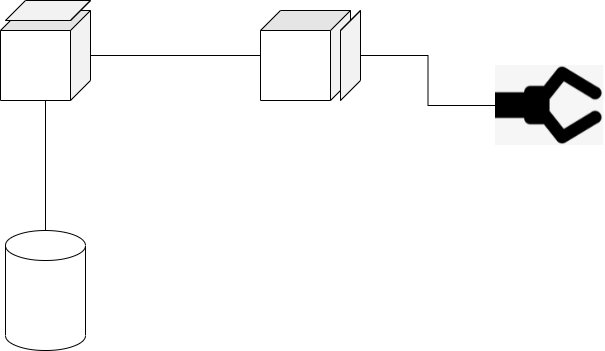
\includegraphics[width=0.6\linewidth]{capitolo3/figure/2Dmodel.png}
\caption{2D schematic representation of the robot}
\label{fig:robot2D}
\end{center}
\end{figure}

To apply a kinematic analysis let's consider an open-chain manipulator constituted by $n + 1$ links connected by $n$ joints, where Link 0 is conventionally fixed to the ground and assume that each joint provides the mechanical structure with a single DOF, corresponding to the joint variable. Defining a suitable coordinate frame attached to each link, from Link 0 to Link n the coordinate transformation describing the position and orientation of Frame n with respect to Frame 0 is given by:
\[T_n^0(q) = A_1^0(q1)A_2^1(q2)...A_n^{n-1}(qn)\]


A first way to compute direct kinematics is offered by a geometric analysis of the structure of the given manipulator. The effectiveness of a geometric approach to the direct kinematics problem is based on the ability of the person that creates and analyze the model and, in the choice of the correct and most suitable quantities to define the robot properties. Anyway, if the manipulator structure is complex and the number of joints increases, it is preferable to adopt a less direct solution based on a systematic, general procedure known as Denavit-Hartenberg Method.

\subsection{Denavit-Hartenberg Method}
In order to compute the direct kinematics equation for an open-chain manipulator the Denavit-Hartenberg method has been derived. It is based on four steps that has to be performed to obtain the homogeneous transformation matrix, through which it is possible to know the position and orientation of the end effector. 
\begin{itemize}
    \item Assign frames according to the four DH rules.
    \item Create the DH parameter table.
    \item Plug the table values into the Homogeneous Transformation Matrix.
    \item Multiply the matrices together applying the chaining rule.
\end{itemize}


\subsubsection{Frames Assignment}
 The goal is to define the relative position and orientation of each pair of consecutive links. The problem is that of determining two frames attached to the two links and computing the coordinate transformations between them. The easiest solution is to define some rules to be followed to define in a specific way the frames, so that the final mathematical representation can be as simple as possible. These rules are based on the Denavit-Hartenberg convention. To define the frame for a generic link i (frames are always attached to the link and not to the joint), the following passages has to be realized:

\begin{itemize}
    \item Choose axis $z_i$ along the axis of Joint $i+ 1$.
    \item Locate the origin $O_i$ at the intersection of axis $z_i$ with the common normal to axes $z_i-1$ and $z_i$. Also, locate $O_i’$ at the intersection of the common normal with axis $z_i-1$.
    \item Choose axis $x_i$ along the common normal to axes $z_i-1$ and $z_i$ with positive direction from Joint i to Joint i+ 1.
    \item  Choose axis $y_i$ so as to complete a right-handed frame.
\end{itemize}

\begin{figure}[!h]
\begin{center}
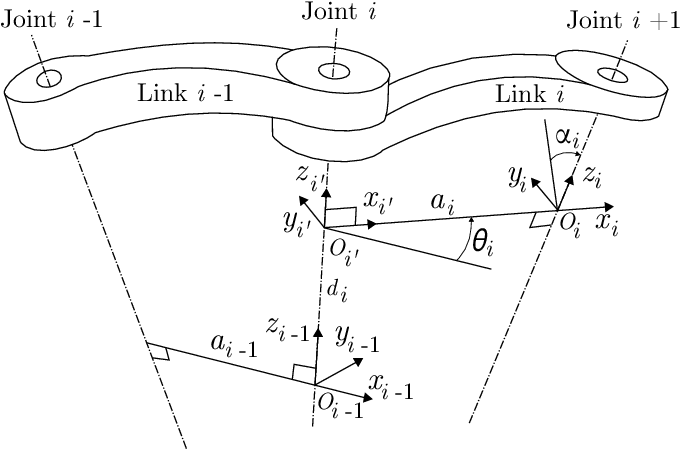
\includegraphics[width=0.6\linewidth]{capitolo3/figure/DHconvention.png}
\caption{Denavit-Hartenberg convention for frame assignment}
\label{fig:DHconvention}
\end{center}
\end{figure}

When defining the frame, notice that it is not true that the reference frame attached to the link has to be in the middle of the object. It could be inside the object but it could be also outside from the physical shape of the object. The only important thing is that the movement of the links is integral with the reference frame, that means that the movements have an effect on the reference frame, i.e. they move in the same way.

The four rules can be rewritten also in a simpler way as follows:
\begin{itemize}
    \item The $Z$ axis must be the axis of revolution, for revolute joint, or the direction of motion, for prismatic joint.
    \item The $X$ axis must be perpendicular to the $Z$ axis of the frame before it.
    \item The $X$ axis must intersect the $Z$ axis of the frame before it.
    \item The $Y$ axis must be drawn so the whole frame follows the right-hand rule.
\end{itemize}

It is also important to notice that are needed at least one more frame than there are joints, since one frame must be on the end-effector. Eventually, it is possible to have also more frames but increasing the number of frames increase also the complexity of the mathematical representation. Before to assign the frame to the link, consider that all axes must be drawn either up, down, right, left, or in the first or third quadrant. This convention is used to obtain a coherent 2D representation in which the axis in the first quadrant represents an axis that goes into the page, whereas the axis in the third quadrant represents an axis that goes out of the page.

Each reference frame is attached to the previous link, so the first one refers to the base of the robot and can be considered as a general fixed reference frame. In order to follow the first Denavit-Hartenberg frame rule the $Z_0$ axis has been assigned so that it coincides with the rotation axis of the revolute joint. For the $X_0$ axis since, in this case, there is not a previous frame it is possible to assign it arbitrarily, without any constraint. Finally, the $Y_0$ axis has to be drawn following the right hand rule, according to the fourth DH frame rule. The final result for the first frame is shown in Figure\ref{fig:first_frame}.

\begin{figure}[!h]
\begin{center}
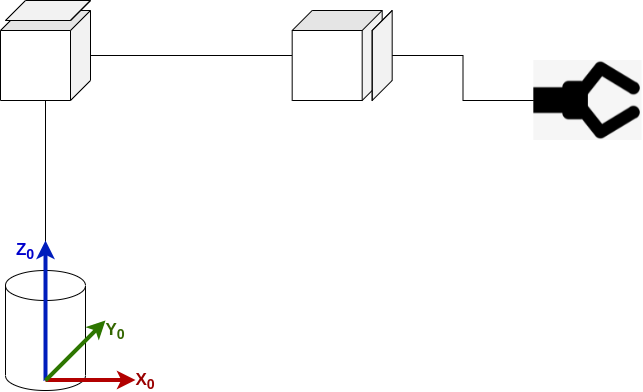
\includegraphics[width=0.6\linewidth]{capitolo3/figure/first_frame.png}
\caption{First reference frame}
\label{fig:first_frame}
\end{center}
\end{figure}

For the second frame, the $Z_1$ axis follows the direction of motion of the prismatic joint and it points up. To define the direction of the $X_1$ now the second and third rule has to be satisfied. For this reason, it has been chosen toward right so that it is perpendicular to $Z_0$ and, prolonging $Z_0$ and $X_1$, they intersect. The $Y_1$ axis follows the right hand rule. The final result for the second frame is shown in Figure\ref{fig:second_frame}.

\begin{figure}[!h]
\begin{center}
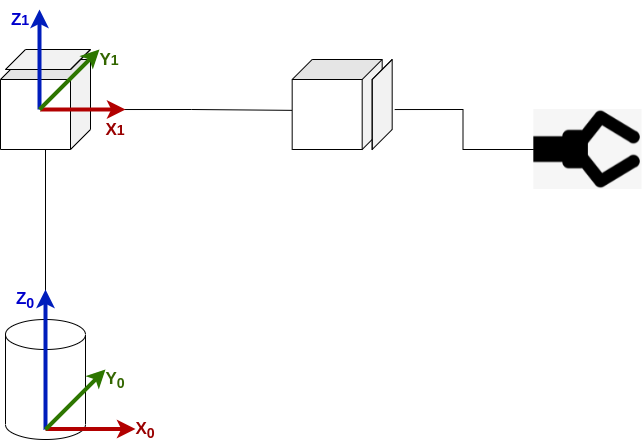
\includegraphics[width=0.6\linewidth]{capitolo3/figure/second_frame.png}
\caption{Second reference frame}
\label{fig:second_frame}
\end{center}
\end{figure}

In the third frame, the $Z_2$ axis follows the direction of motion of the second prismatic joint. Then, since the $X_2$ axis must be perpendicular to the $Z_1$ axis, it can not be drawn up or down because in this case it would be parallel and can not be drawn right or left because it has to be perpendicular also to its own $Z_2$ axis. So, it points out of the page. However, it does not respect the third DH rule because the $X_2$ axis and the $Z_1$ axis does not intersect. To solve this kind of problem, it is possible to translate the reference frame, as a first option, and if this does not solve the issue a rotation of the frame has to be applied. The first solution is preferable because it does not change the mutual position of the current frame with the previous ones. In this case translating the third reference frame, so that its origin coincides with the one of the second frame, is enough to solve the problem. The $Y_2$ axis follows the right hand rule. The final result for the third frame is shown in Figure\ref{fig:third_frame}.

\begin{figure}[!h]
\begin{center}
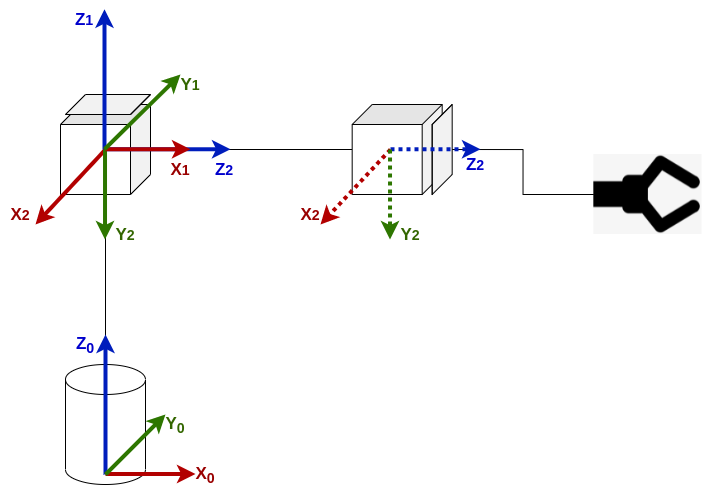
\includegraphics[width=0.6\linewidth]{capitolo3/figure/third_frame.png}
\caption{Third reference frame}
\label{fig:third_frame}
\end{center}
\end{figure}

The last frame is attached to the end effector, and is generally addressed as end-effector frame. Here, there is not a constraint for the $Z_3$ so the best solution is to define it parallel to the previous frame to keep simple the maths. The $X_3$ axis, instead, must be perpendicular to $Z_2$ and should intersect it, so it has been drawn up. The $Y_3$ axis follows the right hand rule. The complete model with all the frames correctly assigned is shown in Figure\ref{fig:complete_frames}.

\begin{figure}[!h]
\begin{center}
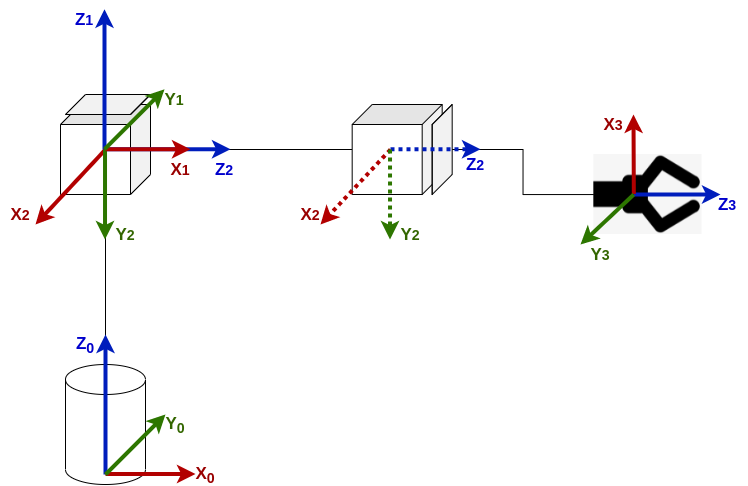
\includegraphics[width=0.6\linewidth]{capitolo3/figure/complete_frames.png}
\caption{Assigned reference frames}
\label{fig:complete_frames}
\end{center}
\end{figure}

\newpage
\subsubsection{DH parameter table}
The second step of the Denavit-Hartenberg method regards the evaluation of the parameters of the robot and the creation of the corresponding DH parameter table. The DH parameter table records all of the displacement and rotation relationship between each pair of frames. As already said, this is important to identify the kinematic of a robot that can be obtained chaining the relation between the reference frames, that are related to translations and rotations. 
Inside the table there are a certain number of columns and rows. 
The columns are always four: two are related to rotations and the other two are related to displacements. 
The number of rows, instead, varies according to the analyzed robot. In particular, if N is the number of frames, the number of rows will be N-1 just because each row will represent information that put in relation two adjacent frames. In this case, there are four frames so the table will have three rows. The application of the DH convention described before allows to minimize the number of parameters needed. Actually, only two parameters for the rotation and two parameters for the displacement are needed. So, having this parameters for each pair of frames the homogeneous transformation matrix can be directly derived.

In particular, the four parameters are:
\begin{itemize}
    \item \textbf{$\theta$}. It is the amount we have to rotate frame n-1 around the axis $Z_n -1$ in order to get axis $X_n -1$ to match the axis $X_n$. 
    
    \begin{figure}[!h]
    \begin{center}
    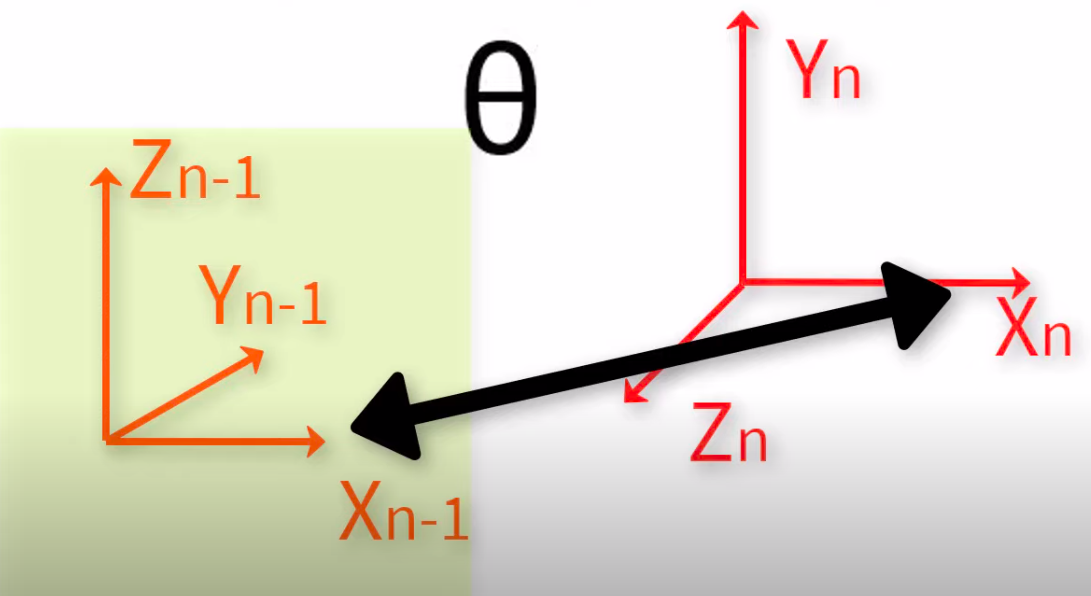
\includegraphics[width=0.5\linewidth]{capitolo3/figure/theta.png}
    \caption{First rotational parameter}
    \label{fig:theta}
    \end{center}
    \end{figure}

    Moreover, any rotation of the joint has to be included if the joint is a revolute one, because this rotation is also a rotation around the axis $Z_n -1$. The value of $\theta$ is composed by two elements:
    \begin{itemize}
        \item A static part. For construction we could have a static offset, so in this case a rotation to align the two X axis has to be applied.
        \item A dynamic part. If the frame is placed on a revolute joint also the rotation has to be considered. If the revolute joint rotates, it will change the orientation of each link, and the orientation of each reference frame attached to the other elements of the robot, and this could create a relative angle between the two adjacent axis.
    \end{itemize}
 
     At the end, the correct value is obtained adding the static offset and the dynamic effect of the joint. This last contribute is coincident with the angle of rotation of the joint that is considered to be positive if the rotation is counter-clockwise.
 
    \item \textbf{$\alpha$}. The angle of rotation of frame n-1 around $X_n$ in order to align the two $Z$ axis.
    
    \begin{figure}[!h]
    \begin{center}
    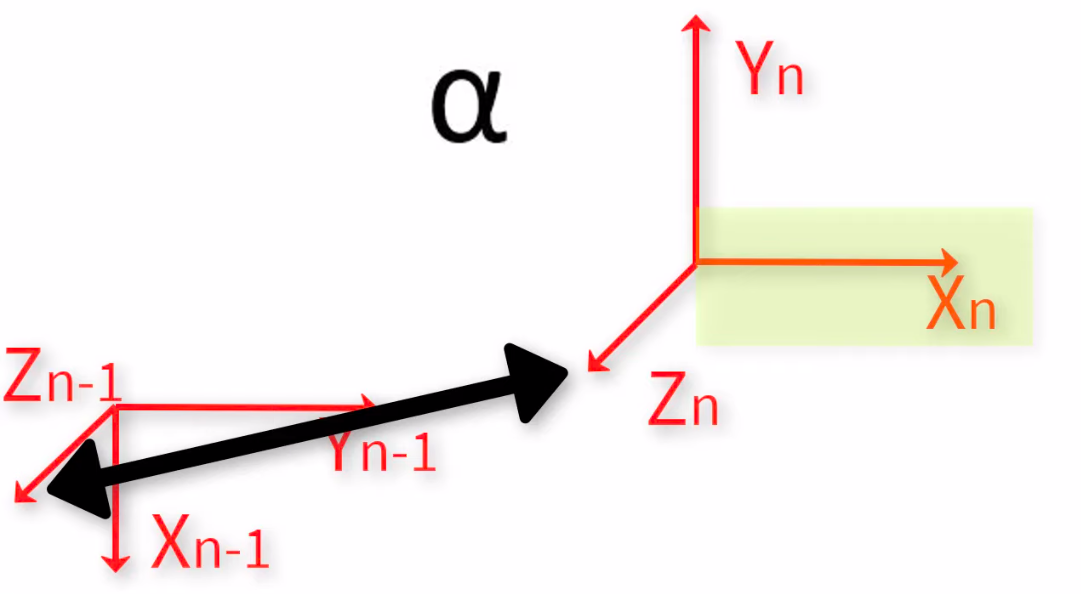
\includegraphics[width=0.5\linewidth]{capitolo3/figure/alpha.png}
    \caption{Second rotational parameter}
    \label{fig:alpha}
    \end{center}
    \end{figure}
    
    The axis $X_n$ is fixed and the plane $X_{n-1}Z_{n-1}$ rotates in order to align $Z_n$ and $Z_{n-1}$. To know the sign of the rotation angle the right hand rule is used. So, putting the thumb in the direction of $X$ (now the $X$ is the rotation axis) it is possible to verify in which direction the other fingers, that are aligned with the $Z_{n-1}$ rotate. If the rotation is performed clockwise the sign is negative, if counterclockwise the value of $\alpha$ is positive. For the alpha column, the rotation due to the actuator does not produce any effect on the mutual orientation between the frames, so it is not needed to consider the dynamic part related to the effect of the rotation of the revolute joint.
    \item \textbf{r}. The first displacement parameter is the amount of displacement from the centre of the reference frame n-1 to the centre of the frame n, measured only in the $X_n$ direction.
    \begin{figure}[!h]
    \begin{center}
    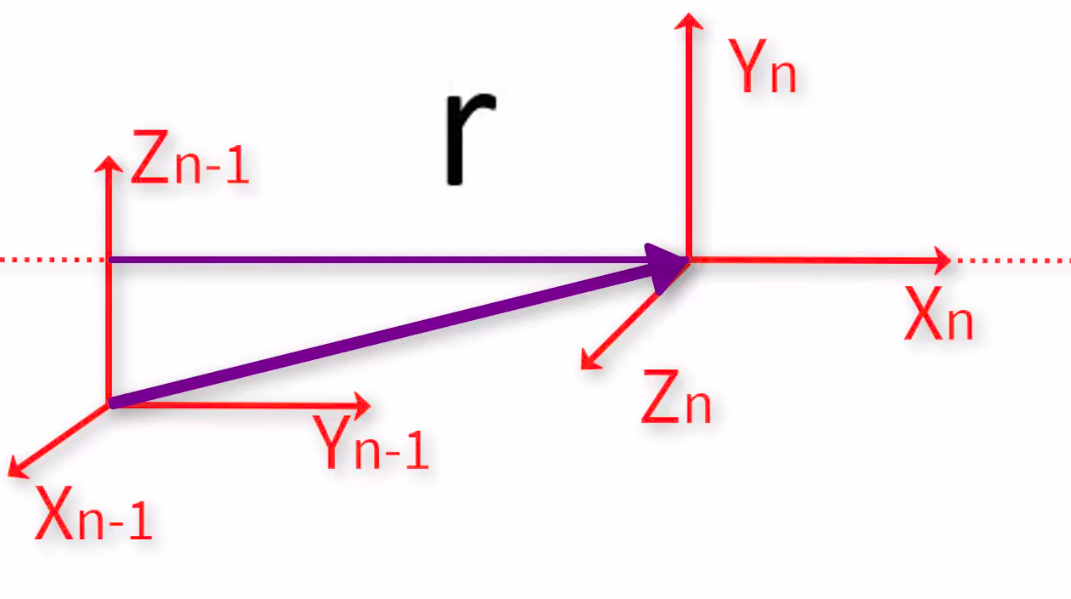
\includegraphics[width=0.5\linewidth]{capitolo3/figure/r.png}
    \caption{First displacement parameter}
    \label{fig:r}
    \end{center}
    \end{figure}
    
    \item \textbf{d}. It is the amount of displacement from the centre of frame n-1 to the centre of frame n, measured only in the $Z_n-1$ direction.
    \begin{figure}[!h]
    \begin{center}
    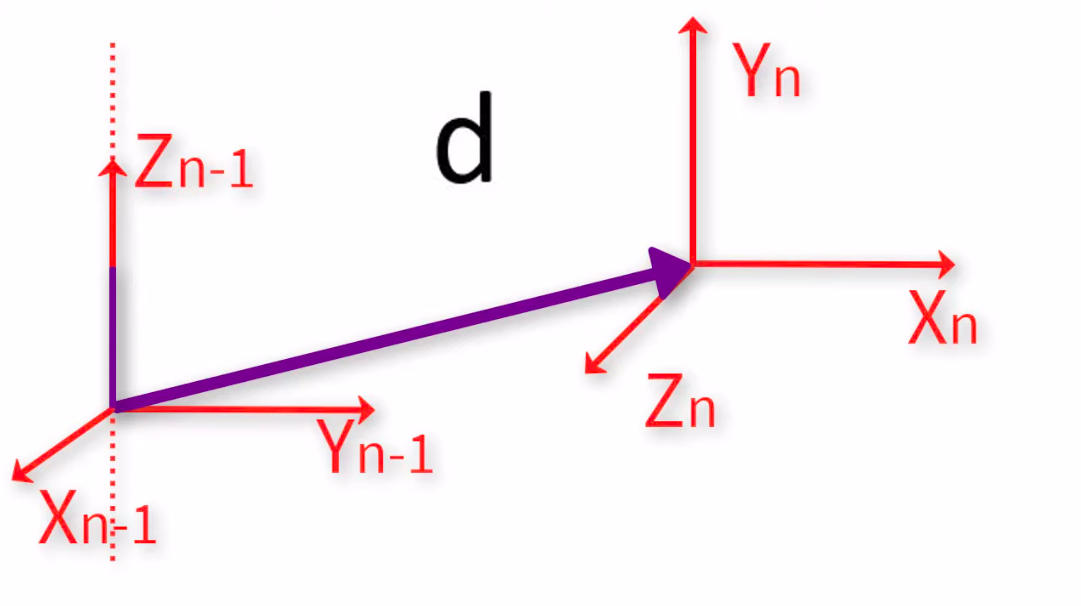
\includegraphics[width=0.5\linewidth]{capitolo3/figure/d.png}
    \caption{Second displacement parameter}
    \label{fig:d}
    \end{center}
    \end{figure}
\end{itemize}

\newpage
For our robot, the DH parameter table is the following:

%\begin{table}[!htp]\centering
%\caption{Denavit-Hartenberg parameter table}\label{tab:DH_table}
%\scriptsize
%\rowcolors{1}{}{tablelightgray}
%\begin{tabular}{lcccc}\toprule
%$\theta$ &$\alpha$ &r &d\\\midrule
%0+ \theta_1 &0 &0 &$a_1$ \\
%$-90^{\circ}$&$-90^{\circ}$&0&$0 + d_1$  \\
%$-90^{\circ}$&0&$a_4$&$a_2+a_3+d_2$ \\
%\bottomrule
%\end{tabular}
%\end{table}

\begin{longtable}{|p{3cm}|p{3cm}|p{3cm}|p{3cm}|}
	\hline 
	\textbf{$\theta$}&\textbf{$\alpha$}&\textbf{r}&\textbf{d}\\ 
	\hline 
	$0+ \theta_1$&0&0&$a_1$\\ 
	\hline
    $-90^{\circ}$&$-90^{\circ}$&0&$0 + d_1$\\
	\hline
	$-90^{\circ}$&0&$a_4$&$a_2+a_3+d_2$\\
	\hline
	\caption{Denavit-Hartenberg parameter table}
    \label{table:DHtable}
\end{longtable} 

% d1 è solo non negativa
% d2 al max 9
% a1 18.5
% a2 =0
% a3 dal centro dell'asse orizzontale al centro del gripper

Let's consider the parameter $\theta$. The rotation of frame zero around $Z_0$ to align $X_0$ and $X_1$ is equal to zero since they are already aligned, but the dynamic component related to the rotation of the revolute joint ($\theta_1$) is then added. The rotation of frame 1 around $Z_1$ in order to get axis $X_1$ to match the axis $X_2$ is equal to $90^{\circ}$. The sign is negative because we rotate clockwise. Also the rotation of frame 2 around $Z_2$ in order to get axis $X_2$ to match the axis $X_3$ is equal to $-90^{\circ}$.

The $\alpha$ parameters have been derived as follows. The angle of rotation of frame zero around $X_1$ in order to align the two $Z$ axes is zero because they are already aligned. The angle of rotation of frame 1 around $X_2$ to align $Z_1$ and $Z_2$ is $-90^{\circ}$ because the rotation is clockwise. Then, axes $Z_2$ and $Z_3$ are aligned, so the last angle $\alpha$ is zero.

Considering the $r$ parameter, the displacement between the origin of frame 0 and frame 1 measured along the $X_n$ is zero. The distance between the origins of frame 1 and frame 2 is zero because they coincide. The displacement between the origin of frame 2 and the origin of frame 3 is reported in figure \ref{fig:DHparameters} as an orange arrow. Its projection on the $X_3$ axis is the segment indicated with $a_4$.

\begin{figure}[!h]
\begin{center}
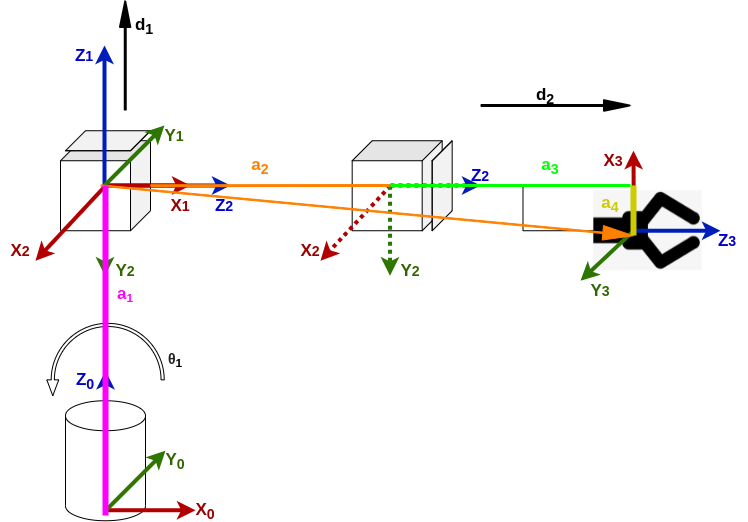
\includegraphics[width=0.7\linewidth]{capitolo3/figure/DHparameter.png}
\caption{DH parameter}
\label{fig:DHparameters}
\end{center}
\end{figure}

The displacement $d$ between frame 0 and frame 1 measured on the $Z_0$ axis is the segment $a_1$ (see figure \ref{fig:DHparameters}). The distance between $O_1$ and $O_2$ is null because they coincide but the dynamic component $d_1$ related to the prismatic joint motion has to be added. The distance between $O_2$ and $O_3$ along $Z_2$ is the sum of $a_2$ (dimension of the second link), $a_3$ (dimension of the third link) and $d_2$ that is the dynamic component of the second prismatic joint.

\newpage
Substituting the value physically measured on the robot we obtain the table \ref{table:DHtable1}.

\begin{longtable}{|p{3cm}|p{3cm}|p{3cm}|p{3cm}|}
	\hline 
	\textbf{$\theta$}&\textbf{$\alpha$}&\textbf{r (\SI{}{\centi\metre})}&\textbf{d (\SI{}{\centi\metre})}\\ 
	\hline 
	$\theta_1$&0&0&$18.5$\\ 
	\hline
    $-90^{\circ}$&$-90^{\circ}$&0&$d_1$\\
	\hline
	$-90^{\circ}$&0&$6.75$&$20+d_2$\\
	\hline
	\caption{Denavit-Hartenberg parameter table}
    \label{table:DHtable1}
\end{longtable} 

The length of the second link $a_2$ is equal to zero since the third frame has been moved in the same point of the second frame. The link between the second prismatic joint and the gripper is around 20 \SI{}{\centi\metre}.

\subsubsection{Homogeneous Transformation Matrix}
In order to achieve a compact representation of the relationship between the coordinates of the same point in two different frames, the homogeneous representation of a generic vector p can be introduced as a new vector formed by adding a fourth unit component. This new way to represent the points allows to avoid in the mapping between two generic points p0 and p1, the presence of an additive term and it is possible just to condensate this mapping into a new matrix A, the homogeneous transformation matrix. 
\newpage
The shape of the new matrix is a block matrix that contains a first block that is the rotation matrix, on the right side there is an other block that is a column that contains the three components of the vector $O_1^0$ that is the displacement between the two origins. The last row is composed by a vector of zeros and a term equal to one.

At this point, it is possible to express the coordinate transformation between each pair of frame $i$ and $i-1$.

\begin{equation}
    A_i^{i-1}(q_i) =  A_i'^{i-1} A_i^{i'} = 
    \begin{bmatrix}
    c_{\theta_i} & -s_{\theta_i}c_{\alpha_i} & s_{\theta_i}s_{\alpha_i} &r_i c_{\theta_i}\\
    s_{\theta_i} & c_{\theta_i}c_{\alpha_i} & -c_{\theta_i}s_{\alpha_i} &r_i s_{\theta_i}\\
     0 & s_{\alpha_i} & c_{\alpha_i} &d_i\\
    0&0&0&1
    \end{bmatrix}
\end{equation}

Matrix frame 0 frame 1.
\begin{equation}
    A_1^{0}(q_1) = 
    \begin{bmatrix}
    c_{\theta_1} & -s_{\theta_1} & 0 &0\\
    s_{\theta_1} & c_{\theta_1} & 0 &0\\
     0 & 0 & 1 &18.5\\
    0&0&0&1
    \end{bmatrix}
\end{equation}

Matrix frame 1 frame 2.
\begin{equation}
    A_2^{1}(q_2) = 
    \begin{bmatrix}
   0 & 0 & 1 &0\\
   -1 & 0 & 0 &0\\
     0 & -1 & 0 &d_1\\
    0&0&0&1
    \end{bmatrix}
\end{equation}

Matrix frame 2 frame 3.
\begin{equation}
    A_3^{2}(q_3) = 
    \begin{bmatrix}
r   0 & 1 & 0 &0\\
   -1 & 0 & 0 &-6.75\\
     0 & -1 & 0 &20+d_2\\
    0&0&0&1
    \end{bmatrix}
\end{equation}

Complete matrix from frame 0 to frame 3
\begin{equation}
    A_3^{0}(q_3) = 
    \begin{bmatrix}
   0 &  s_{\theta_1}-c_{\theta_1} & 0 & c_{\theta_1} d_1\\
   0 & -c_{\theta_1}-s_{\theta_1} & 0 &d_1s_{\theta_1}\\
     1 & 0 & 0 &d_1+13.5\\
    0&0&0&1
    \end{bmatrix}
\end{equation}

\section{Hardware setup}

The PLC is used to control the Robot. In particular, the robot use a pinout of 24 pins for inputs and outputs. The pinout, which is shown in Figure\ref{fig:robot_pinout}, describes all the pins which are connected to a particular element of the robot. 

\begin{figure*}[!h]
\centering
\subfloat[Robot Pinout\label{fig:robot_pinout}]{
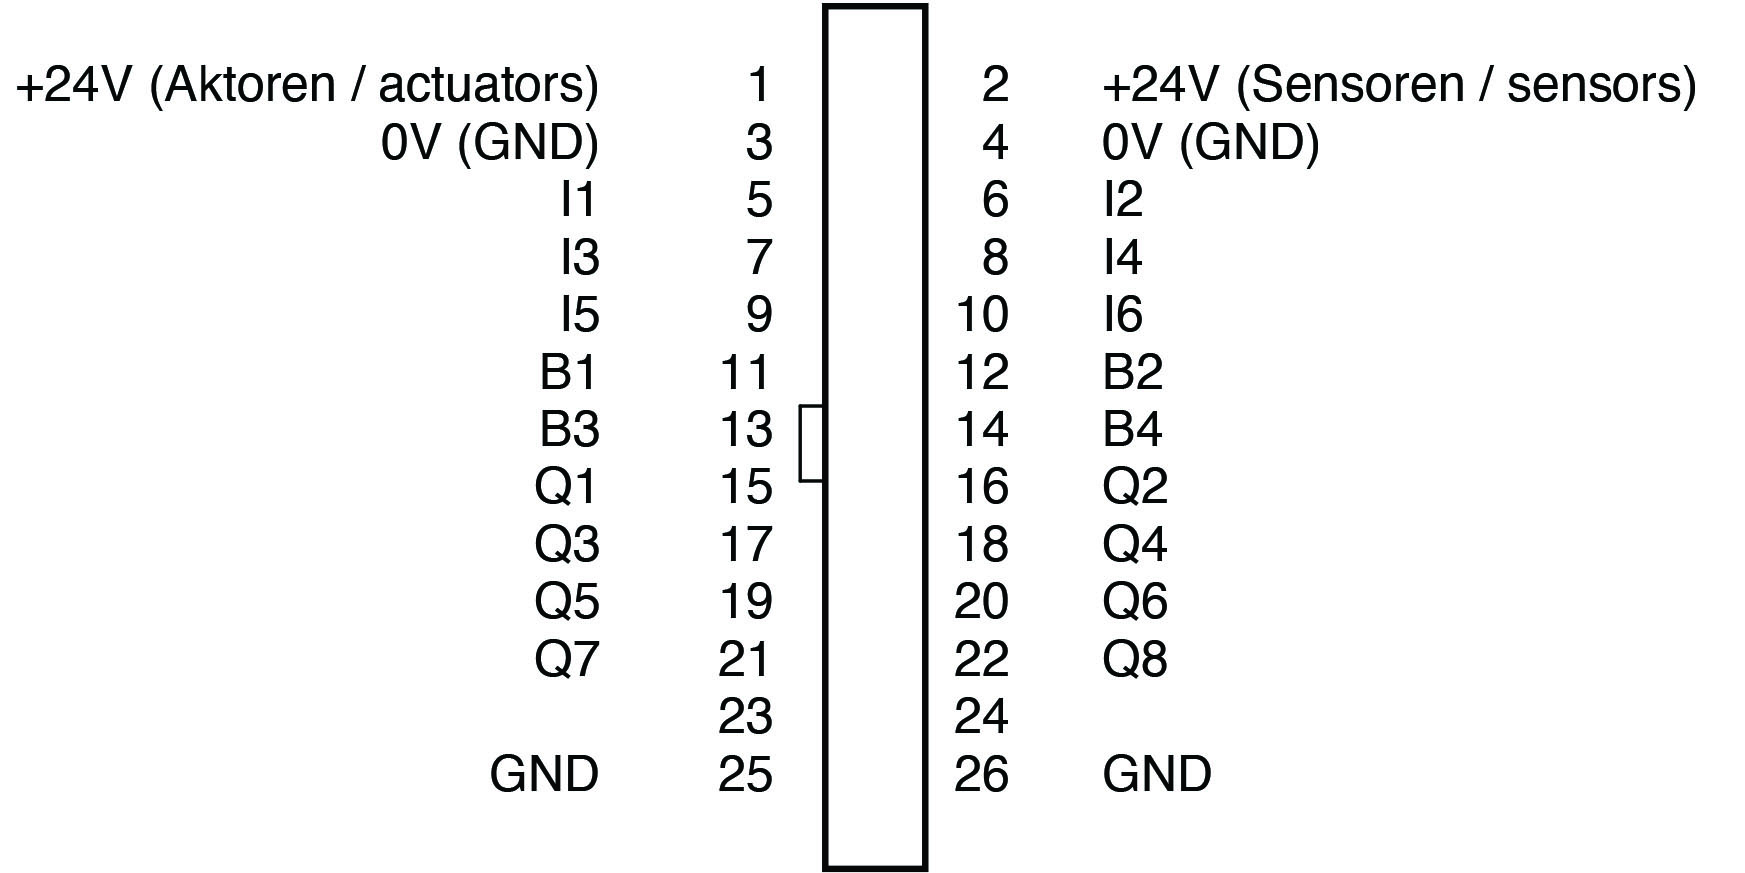
\includegraphics[width=0.45\linewidth]{capitolo3/figure/robot_pinout}
}
\qquad
\subfloat[Photo of Robot Pinout\label{fig:robot_pinout_photo}]{
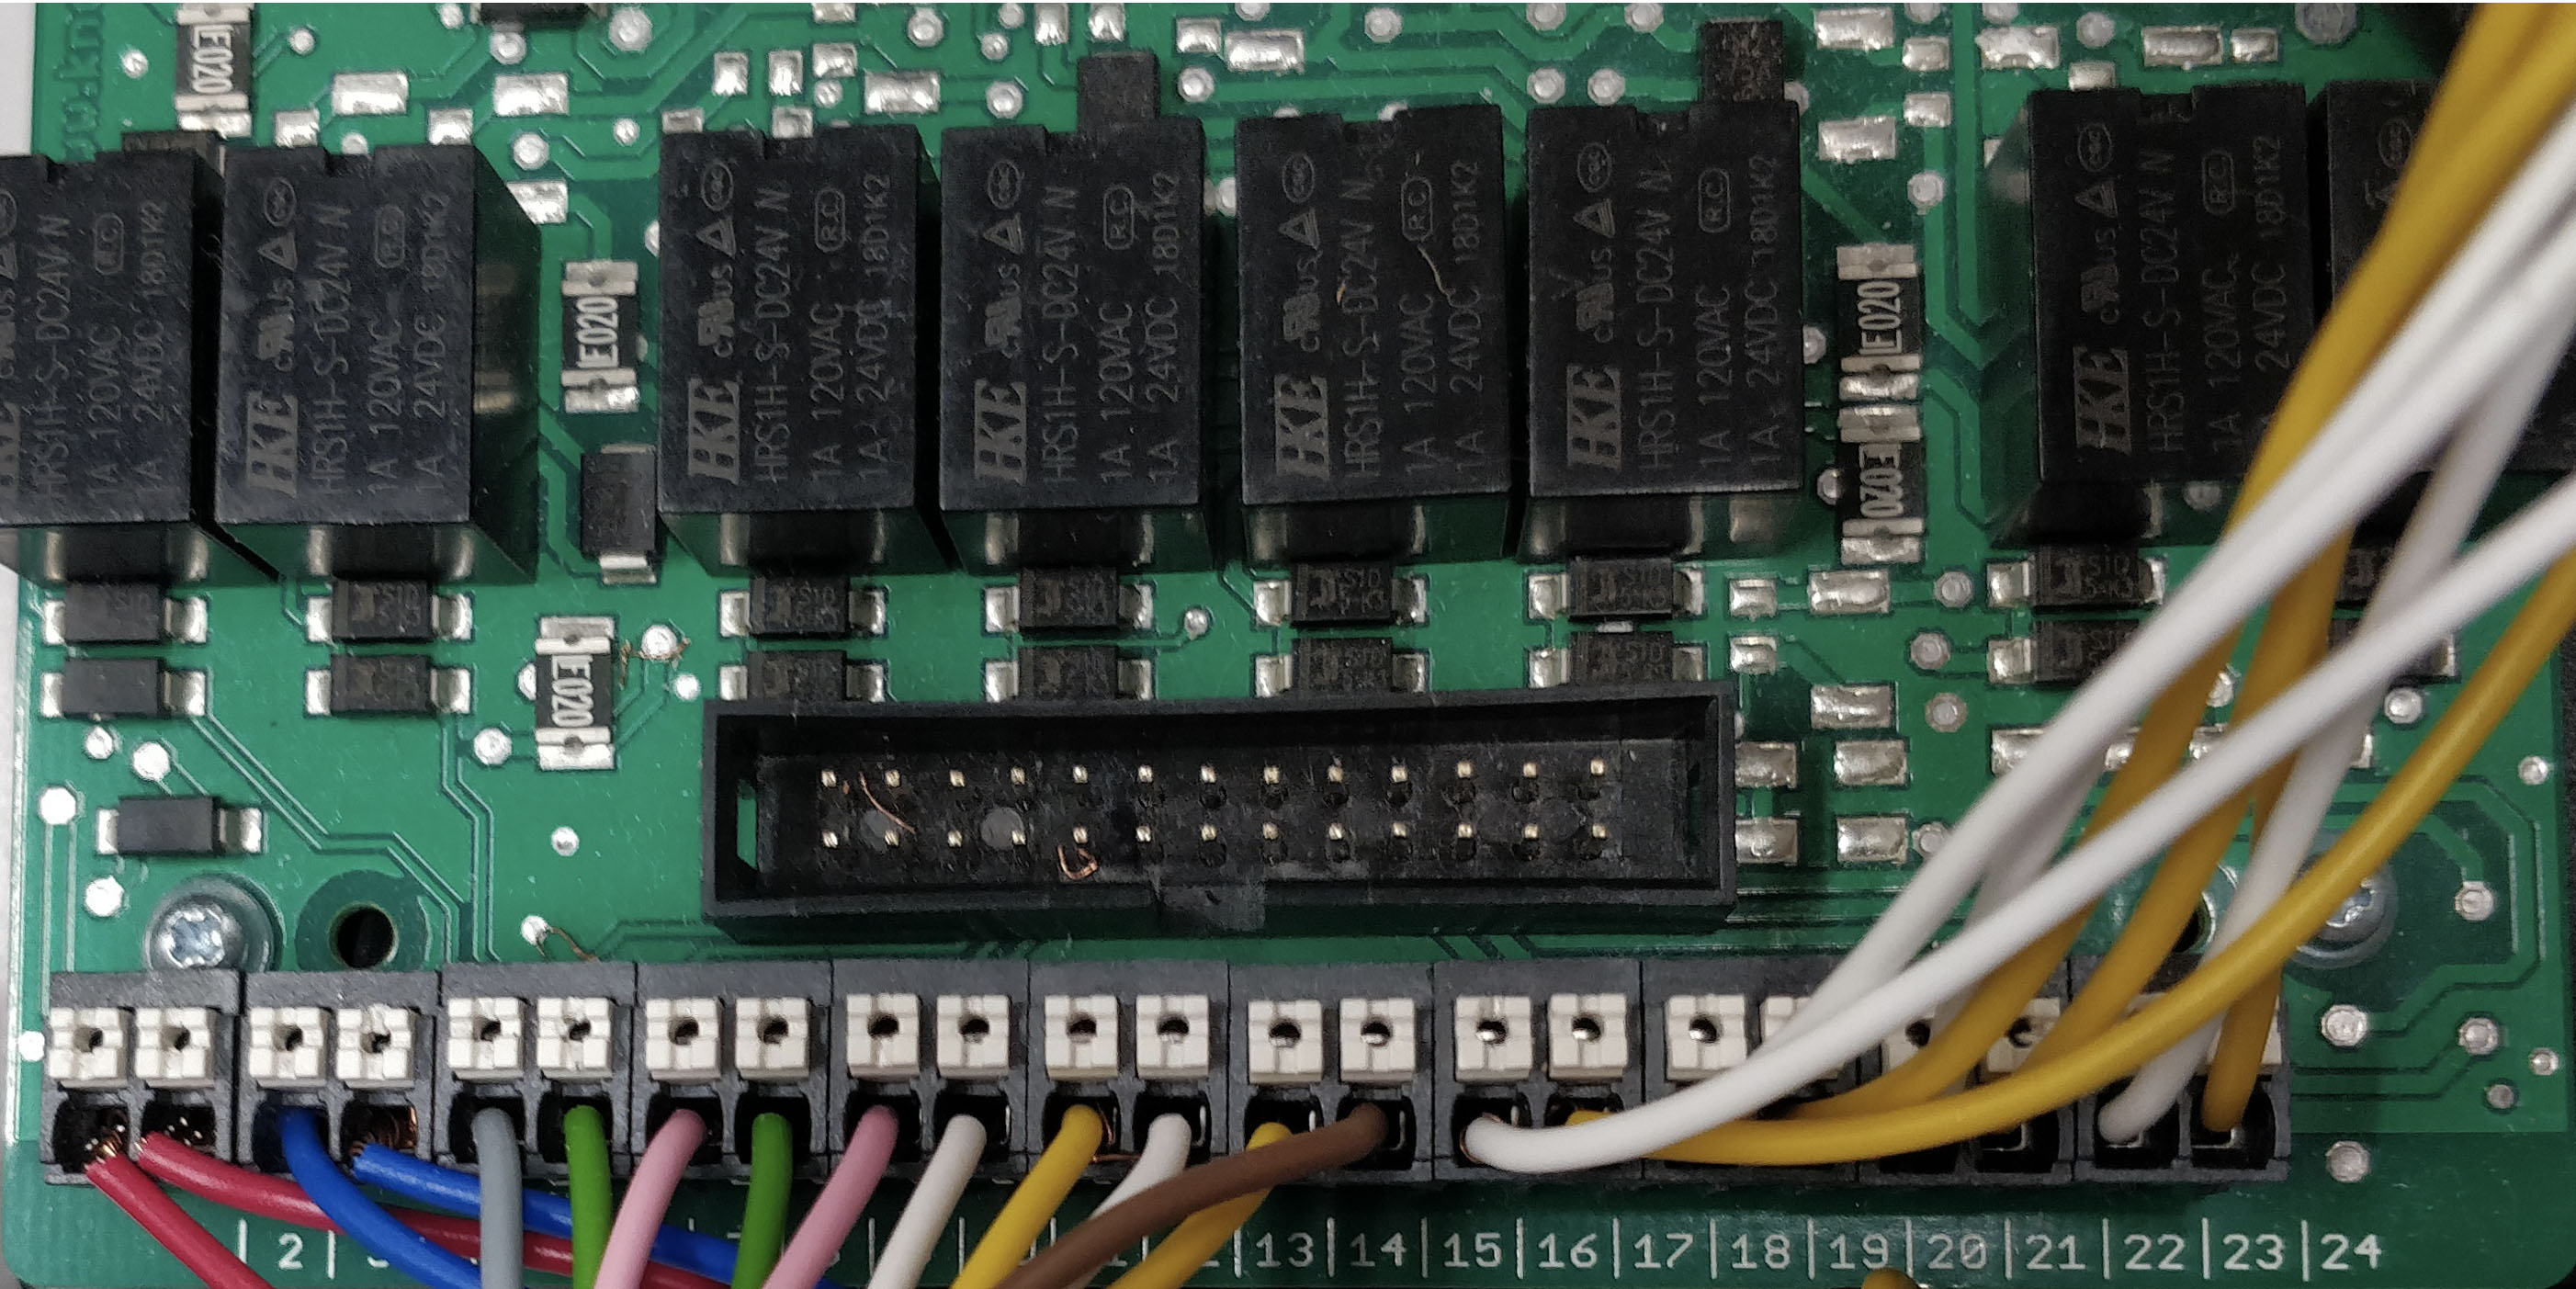
\includegraphics[width=0.45\linewidth]{capitolo3/figure/robot_pinout_photo}
}
\caption{TIA Portal}
\label{first_signal}
\end{figure*}

A more detailed description is presented in the table \ref{tab:robot_pinout_description}, which explains exactly which is the role of each pin. They are detailed the position, a description, the name and the type of pin (input or output).
Moreover, from this table it is also possible to understand how to control each movement of the robot and how to get feedback from it. For example, by powering the terminal number \textbf{15}, it is possible to open the gripper (the end effector) of the robot, while by looking at the status of the pin \textbf{5}, it is possible to know if the gripper is fully open or not.

\begin{table}[!htp]\centering
\caption{Robot pinout description}\label{tab:robot_pinout_description}
\scriptsize
\rowcolors{1}{}{tablelightgray}
\begin{tabular}{lcccc}\toprule
Terminal No. &Function &Pin Name &Robot Input/Output \\\midrule
1 &Power Supply (+) &24V DC &OUTPUT \\
2 &Power Supply (+) &24V DC &OUTPUT \\
3 &Power Supply (-) &0 &OUTPUT \\
4 &Power Supply (-) &0 &OUTPUT \\
5 &Fully Open Gripper &I1 &OUTPUT \\
6 &Pulse Counter Gripper &I2 &OUTPUT \\
7 &Fully Back Arm &I3 &OUTPUT \\
8 &Pulse Counter Back Arm &I4 &OUTPUT \\
9 &Fully Top Arm &I5 &OUTPUT \\
10 &Fully Clockwise Arm &I6 &OUTPUT \\
11 &Encoder Vertical Axis impulse 1 &B1 &OUTPUT \\
12 &Encoder Vertical Axis impulse 2 &B2 &OUTPUT \\
13 &Encoder Turnable Axis impulse 1 &B3 &OUTPUT \\
14 &Encoder Turnable Axis impulse 2 &B4 &OUTPUT \\
15 &Motor Gripper Open &Q1 &INPUT \\
16 &Motor Gripper Close &Q2 &INPUT \\
17 &Motor Arm Front &Q3 &INPUT \\
18 &Motor Arm Back &Q4 &INPUT \\
19 &Motor Arm Down &Q5 &INPUT \\
20 &Motor Arm Up &Q6 &INPUT \\
21 &Motor Rotation Clockwise &Q7 &INPUT \\
22 &Motor Rotation Counter Clockwise &Q8 &INPUT \\
\bottomrule
\end{tabular}
\end{table}

In order to control the robot, the PLC needs to be connected to it. As it is intuitive, the output of the robot (which are useful as feedback for the operations) are connected to the PLC inputs and viceversa. The connection between the two electronic components is depicted with more details in the schematic in Figure\ref{fig:plc_robot_connection} realized with KiCad, a free software suite for electronic design automation (EDA).

\begin{figure}[!h]
\begin{center}
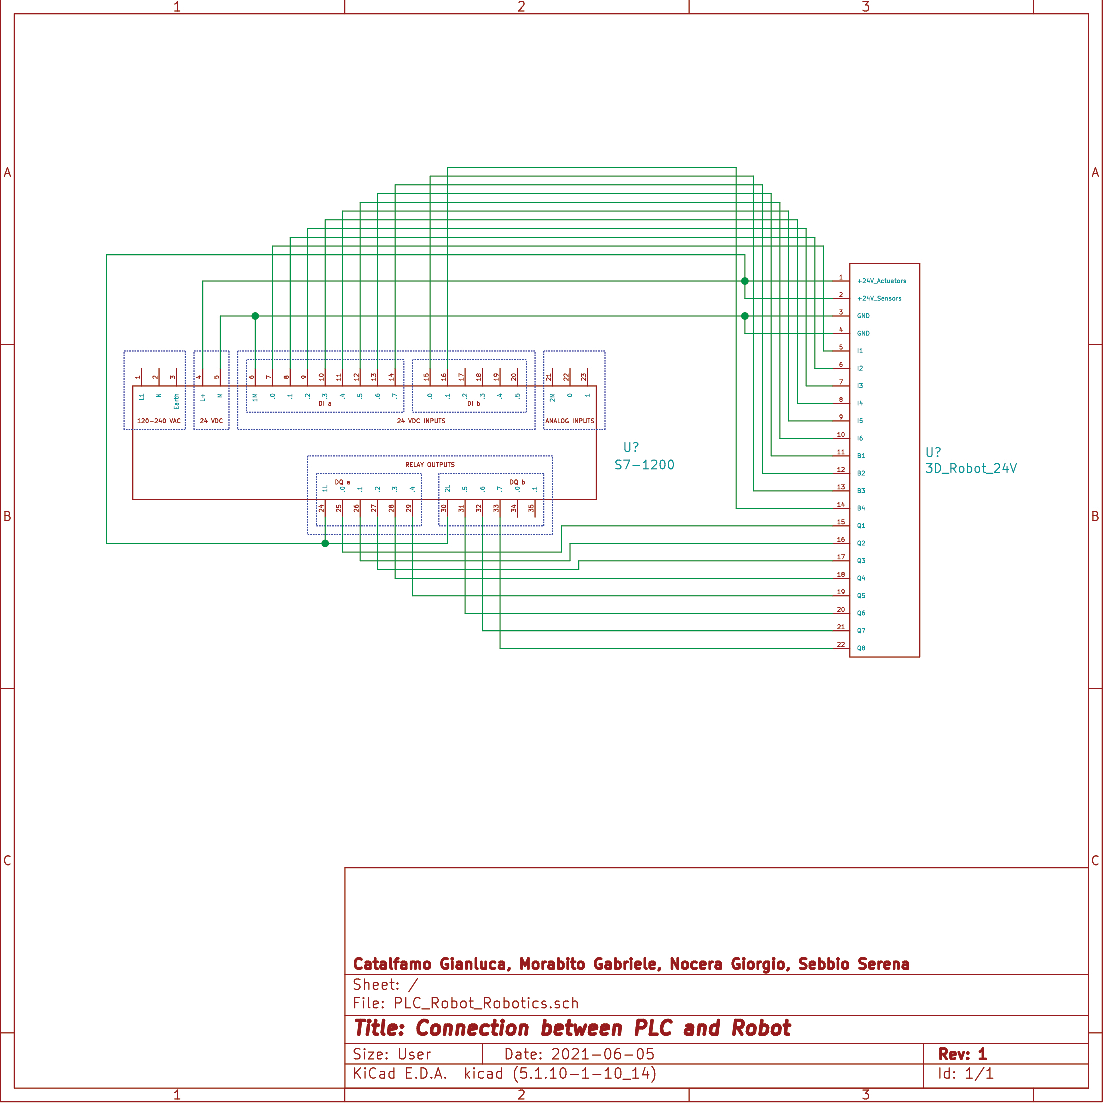
\includegraphics[width=0.8\linewidth]{capitolo3/figure/plc_robot_connection}
\caption{Connection between PLC and Robot}
\label{fig:plc_robot_connection}
\end{center}
\end{figure}

\subsection{First prototype}
For the first version of the prototype the connection shown in Figure\ref{fig:plc_robot_connection} was integrated with a set of 4 buttons, directly connected to the inputs pins \textit{DIb .2} to \textit{.5} of the PLC. This 4 buttons allowed the generation of 16 ($2^4$) possible combinations and, consequently, the possibility to send 16 different signals to the PLC by using only 4 inputs. Even though this system makes them available sixteen combinations, only eight of them were needed to address all the possible moves (Q1 to Q8 on the table \ref{tab:robot_pinout_description}). All the combinations are indicated in the table \ref{tab:moves_combinations}, where under the buttons columns, a value equal to 1 stands for button pressed and viceversa with a value of 0. 
This setup can only be considered as good as a development setup, and it allows to test sensors, motors and combinations before starting the design of the robotic actions.

\begin{table}[!htp]\centering
\caption{Moves combinations}\label{tab:moves_combinations}
\scriptsize
\rowcolors{1}{}{tablelightgray}
\begin{tabular}{lcccccc}\toprule
ID &Button 1 &Button 2 &Button 3 &Button 4 &Operation \\\midrule
1 &0 &0 &0 &0 &None \\
2 &0 &0 &0 &1 &Gripper Open \\
3 &0 &0 &1 &0 &Gripper Close \\
4 &0 &0 &1 &1 &Arm Front \\
5 &0 &1 &0 &0 &Arm Back \\
6 &0 &1 &0 &1 &Arm down \\
7 &0 &1 &1 &0 &Arm Up \\
8 &0 &1 &1 &1 &Rotation Clockwise \\
9 &1 &0 &0 &0 &Rotation Counter Clockwise \\
10 &1 &0 &0 &1 &None \\
11 &1 &0 &1 &0 &None \\
12 &1 &0 &1 &1 &None \\
13 &1 &1 &0 &0 &None \\
14 &1 &1 &0 &1 &None \\
15 &1 &1 &1 &0 &None \\
16 &1 &1 &1 &1 &Reset \\
\bottomrule
\end{tabular}
\end{table}

In Figure \ref{fig:fisrt_proto_schematic} it is possible to see the first prototype schematic.

\begin{figure}[!h]
\begin{center}
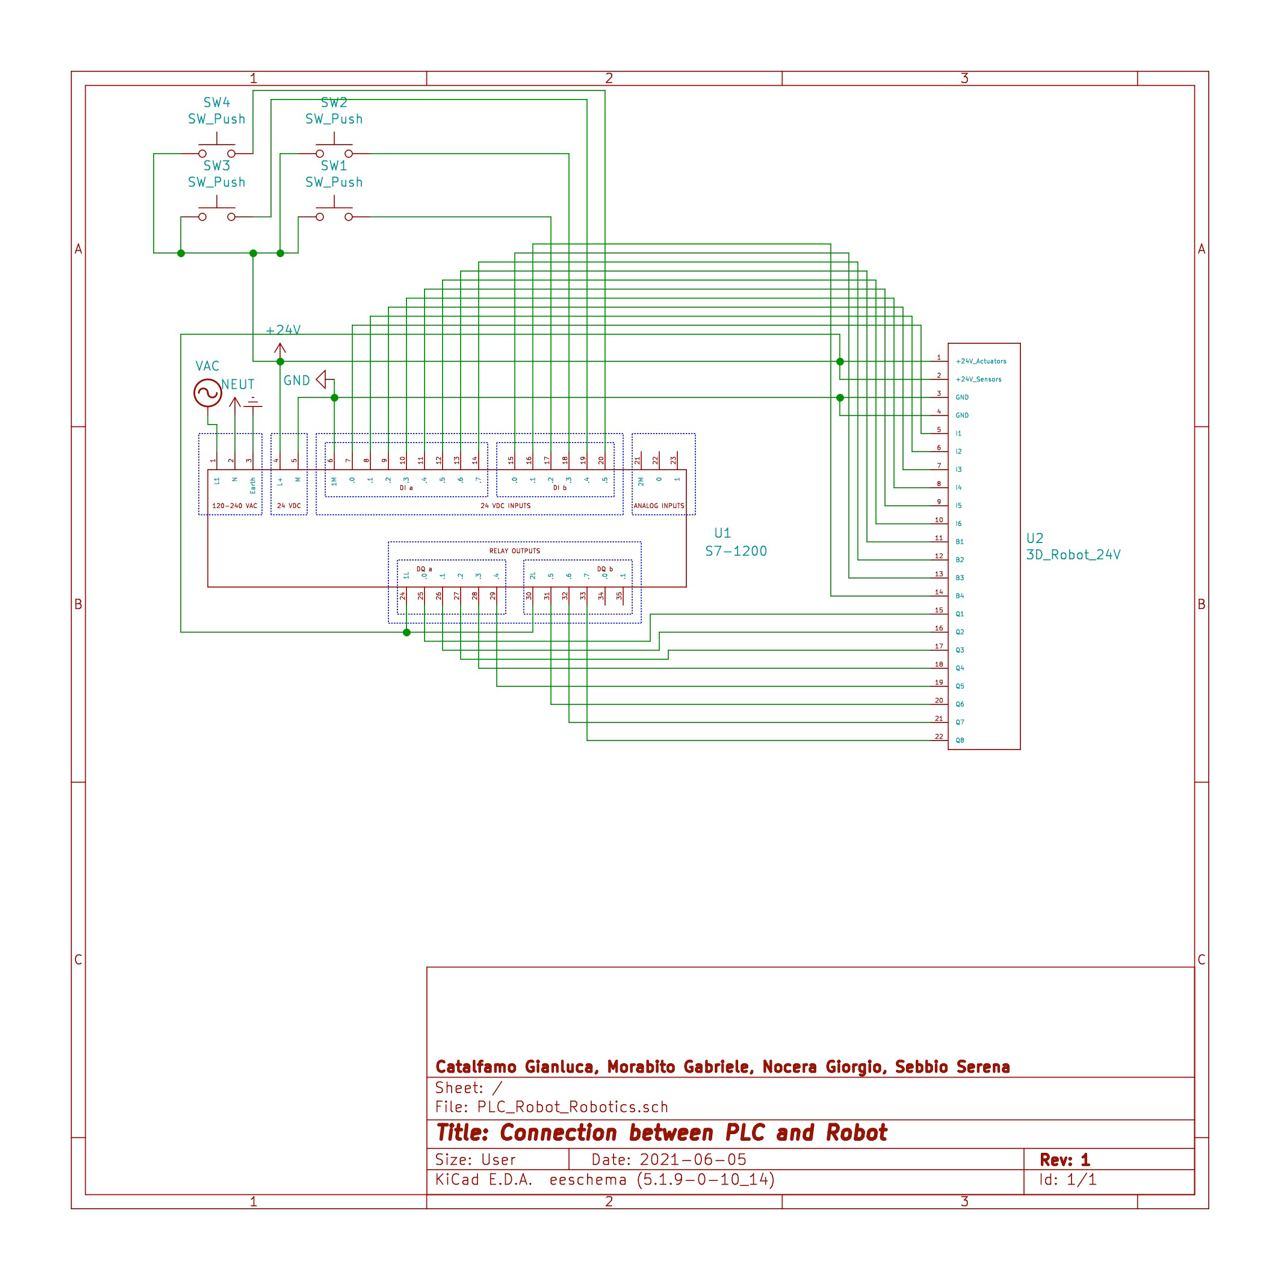
\includegraphics[width=1\linewidth]{capitolo3/figure/first_prototype.png}
\caption{First prototype schematic}
\label{fig:fisrt_proto_schematic}
\end{center}
\end{figure}

\newpage
\begin{figure*}[!h]
\centering
\subfloat[Gripper open\label{fig:proto-go}]{
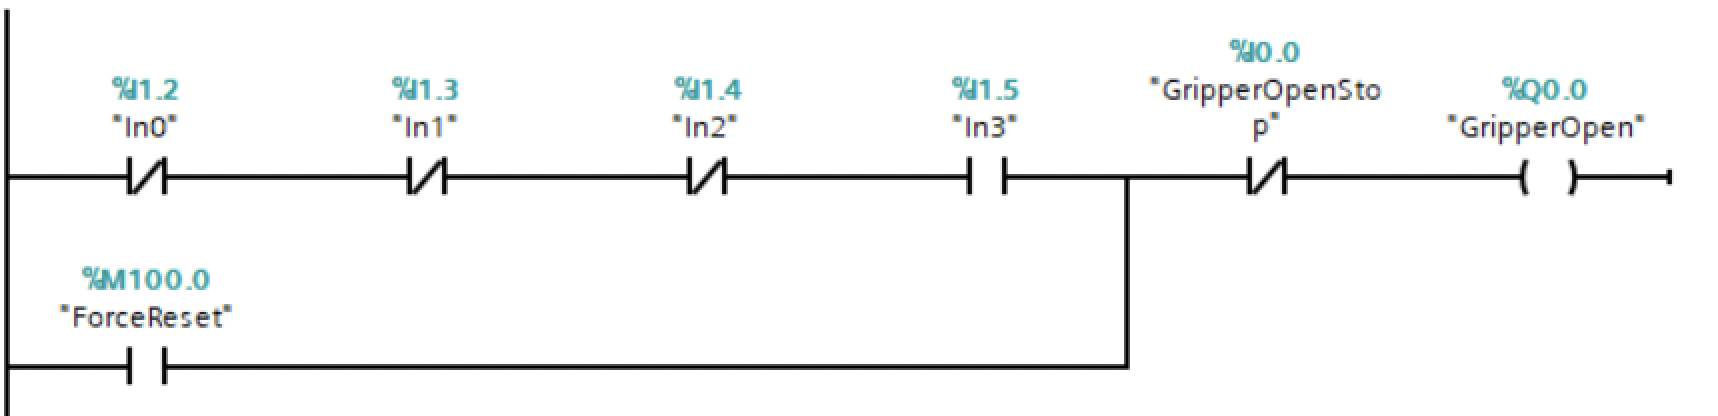
\includegraphics[width=0.4\linewidth]{capitolo3/figure/Prototype_GO.png}
}
\qquad
\subfloat[Gripper close\label{fig:proto-gc}]{
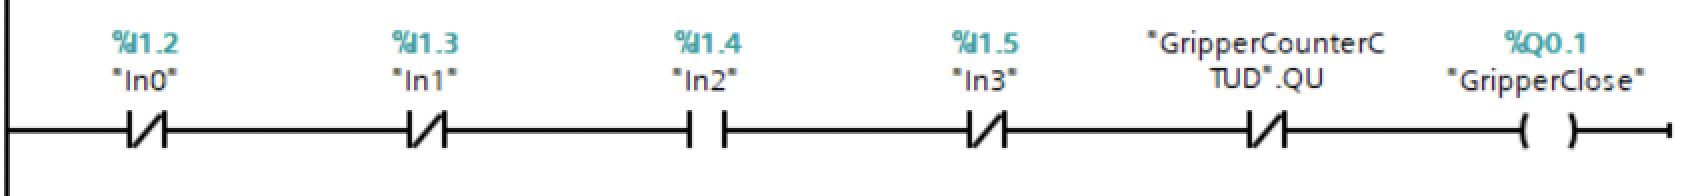
\includegraphics[width=0.4\linewidth]{capitolo3/figure/Prototype_GC.png}
}
\qquad
\subfloat[Arm back\label{fig:proto-ab}]{
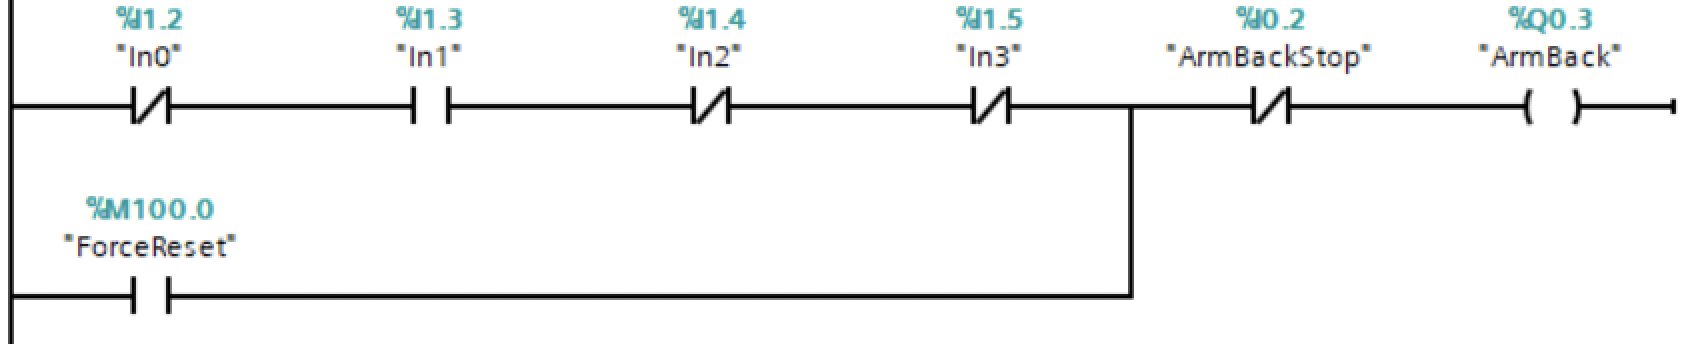
\includegraphics[width=0.4\linewidth]{capitolo3/figure/Protype_AB.png}
}
\qquad
\subfloat[Arm front\label{fig:proto-af}]{
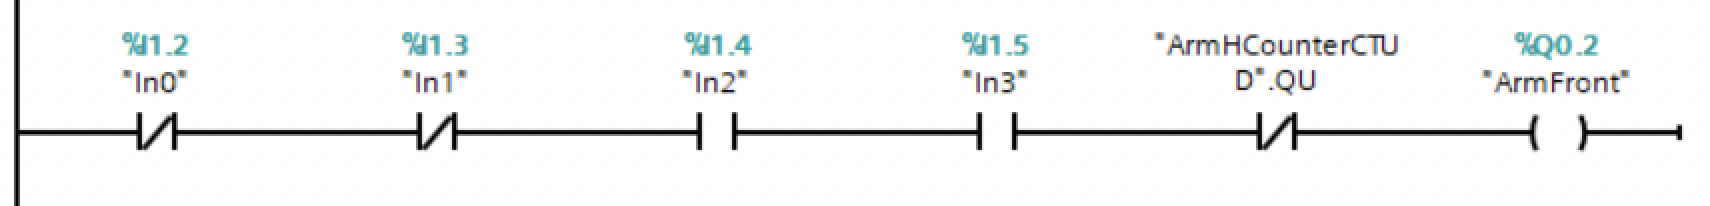
\includegraphics[width=0.4\linewidth]{capitolo3/figure/Protype_AF.png}
}
\qquad
\subfloat[Arm up\label{fig:proto-au}]{
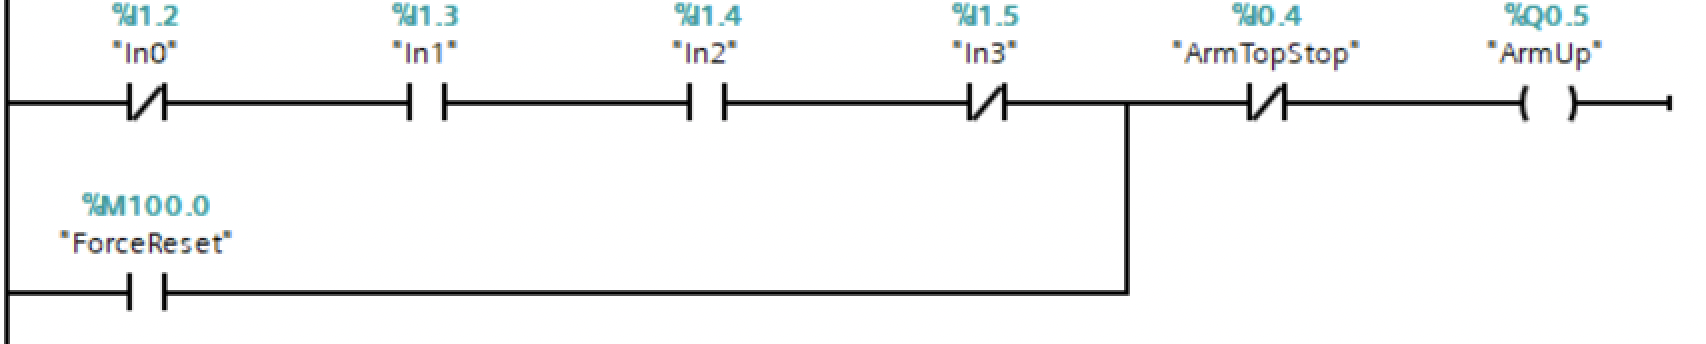
\includegraphics[width=0.4\linewidth]{capitolo3/figure/Protype_AU.png}
}
\qquad
\subfloat[Arm down\label{fig:proto-ad}]{
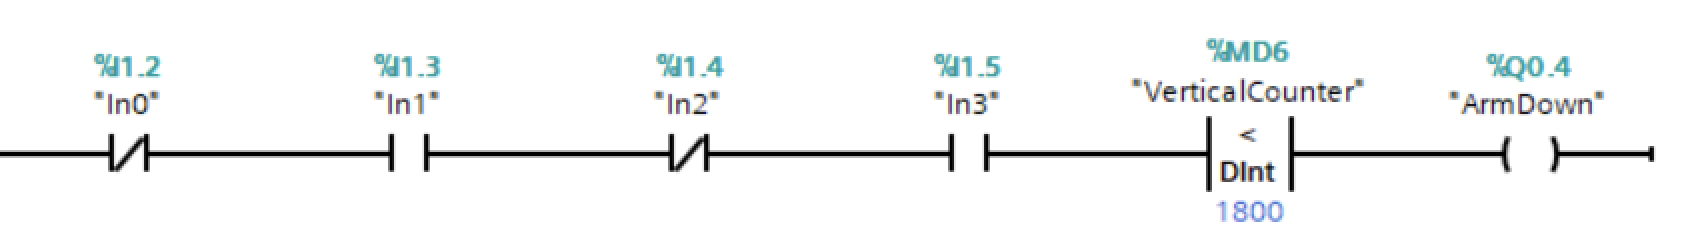
\includegraphics[width=0.4\linewidth]{capitolo3/figure/Prototype_AD.png}
}
\qquad
\subfloat[Rotation clockwise\label{fig:proto-rc}]{
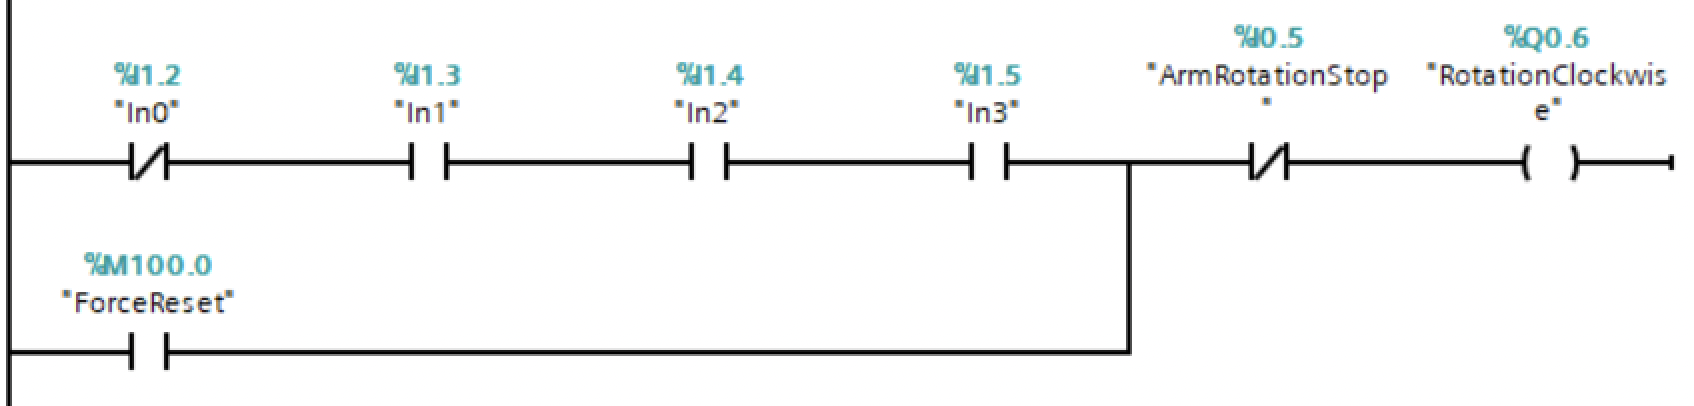
\includegraphics[width=0.4\linewidth]{capitolo3/figure/Prototype_RC.png}
}
\qquad
\subfloat[Rotation counterclockwise\label{fig:proto-rcc}]{
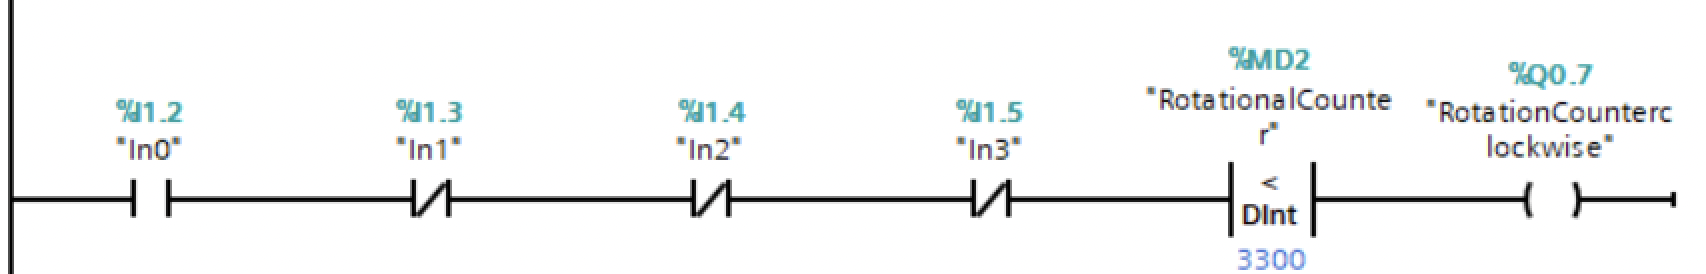
\includegraphics[width=0.4\linewidth]{capitolo3/figure/Prototype_RCC.png}
}
\qquad
\subfloat[Reset\label{fig:proto-reset}]{
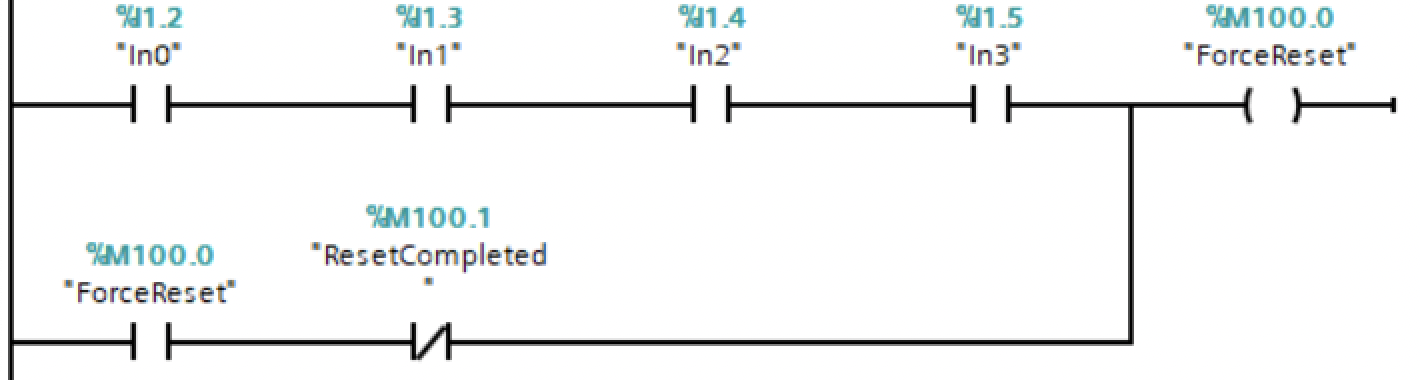
\includegraphics[width=0.4\linewidth]{capitolo3/figure/Prototype_reset.png}
}
\caption{Prototype Ladder Diagram}
\label{fig:proto-ladder}
\end{figure*}

From Figure\ref{fig:proto-ladder} it is possible to see the working conditions explained before. In particular:
\begin{itemize}
    \item In0, In1, In2, In3 correspond respectively to button 1, button 2, button 3 and button 4;
    \item GripperOpenStop, ArmBackStop, ArmTopStop and ArmRotationStop are the variables associated to the corresponding limit switch activation;
    \item the forward movement and the closure of the gripper are stopped if the motor is forced three times, while the counterclockwise rotation and the vertical down movement are stopped when the workspace limit is reached. The details about these stop conditions are explained in section \ref{sec:ladder}, because they were used also in the final implementation. 
\end{itemize}
\textbf{N.B.:} This implementation was realized in order to explore all the functionalities of the robotic arm and of the sensors embedded in it, before realizing the final hardware configuration and programming the PLC.

\subsection{Final Schematic}
The PLC, the robotic arm, the LEDs and the buttons were connected together following the schema in Figure \ref{fig:final_schematic}

\begin{figure}[!h]
\begin{center}
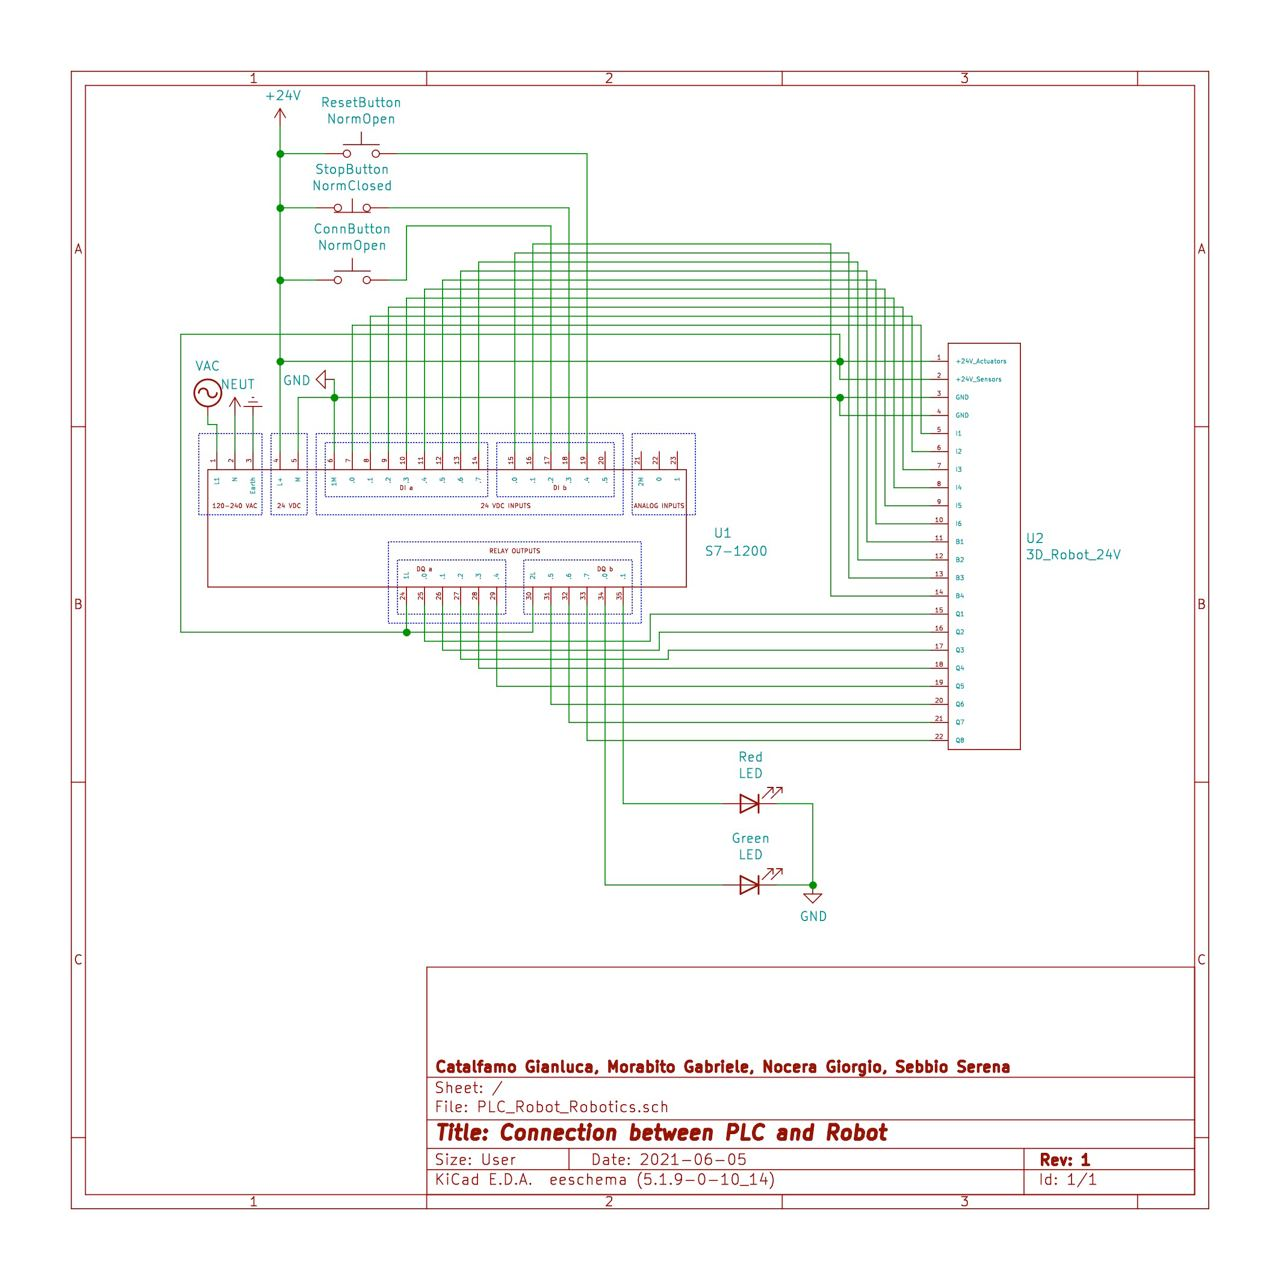
\includegraphics[width=1\linewidth]{capitolo3/figure/final_schematic.png}
\caption{Final schematic}
\label{fig:final_schematic}
\end{center}
\end{figure}

\newpage
\section{Environment setup}

Once the hardware configuration has been completed, to control the movements of the robotic arm a connection between MATLAB and Tia Portal has been set up. This allow a bi-directional communication between the two software so that, the instructions can be launched directly from the command window using some predefined functions and then received and executed by the PLC that send the correct signals to the robotic arm.

\subsection{Establish a TCP connection}

 The TCP connection established requires a master and a slave. In this case MATLAB is master and the PLC is the slave.  
 
\subsubsection{Tia Portal}
First, the correct blocks need to be added in the ladder diagram to control the connection, the disconnection, the send and receive operations. In order to accomplish this task, with the version 15 of Tia Portal, a new segment is added for each of the following blocks:

\begin{itemize}
    \item TCON (Figure\ref{fig:tcon}). The connection block is needed to establish the communication. To add this, go to the "Instructions" tab on the right sidebar, from the list choose the "Communication" section and then from the subsection "Others" drag and drop the TCON block in the newly created segment. Then, right click on the block and choose "Properties" to set the parameters. In the "Configuration" card, for the partner, choose the unspecified option; in the "Connection data" drop down, select new and let the default value in all the other fields. So, the connection ID used in this project, that has to be equal for all the subsequent blocks referring to the same connection will be the default value 1. The port will be the number 2000. Then specify the IP address of the PLC partner, i.e. the address of the computer running the MATLAB instance. To do this, physically connect the PLC to the computer with the Ethernet cable and start the connection from Tia Portal software. Then, the "ipconfig" command has been launched in the command prompt to retrieve the ip address. For this project, the ip address of the PLC is 192.168.0.1 and the one for the computer is 192.168.0.241. To the input port REQ of the TCON block a memory address has to be assigned so, define a bool variable inside the variable table choosing the first address one not already used and then map the tag to the input port. 
    
    \begin{figure}[!h]
    \begin{center}
    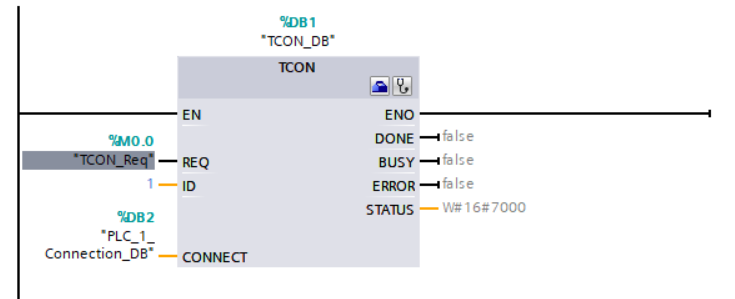
\includegraphics[width=0.8\linewidth]{capitolo3/figure/tcon.PNG}
    \caption{TCON function for the TCP connection}
     \label{fig:tcon}
    \end{center}
    \end{figure}
    
    \item TDISCON (\ref{fig:tdiscon}). This function is used for terminating a TCP connection. Drag and drop the block from the same section seen for the connection function and define in the variable table the tag fro the REQ input that will be again a bool variable with a different and subsequent memory address with respect to the one defined for the connection function. Keep the same value for the connection ID.
\begin{figure}[!h]
    \begin{center}
    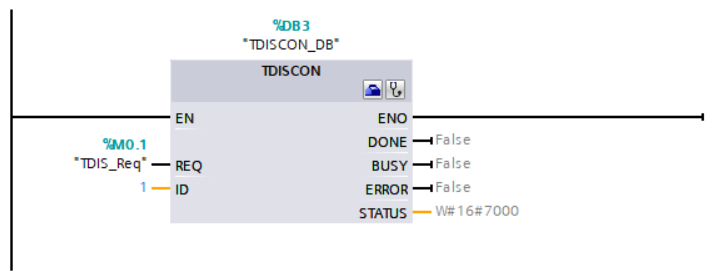
\includegraphics[width=0.8\linewidth]{capitolo3/figure/tdiscon.PNG}
    \caption{TDISCON function the for TCP connection}
    \label{fig:tdiscon}
    \end{center}
\end{figure}
    
    \item TSEND (Figure\ref{fig:tsend}). The function that sends the data from PLC to the TCP partner. For the REQ input port let's define the bool variable with its own memory address. The input port "DATA" is the source from which data is sent.
    
\begin{figure}[!h]
    \begin{center}
    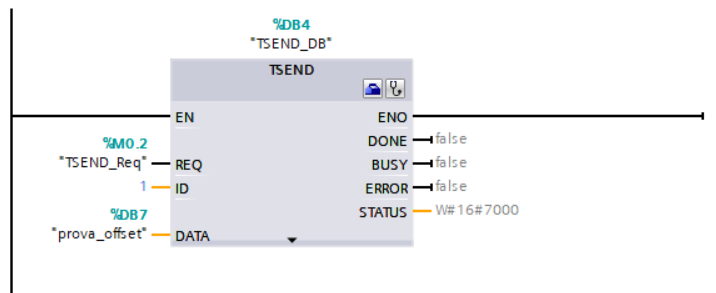
\includegraphics[width=0.8\linewidth]{capitolo3/figure/tsend.PNG}
    \caption{TSEND function the for TCP connection}
    \label{fig:tsend}
    \end{center}
\end{figure}
    
    \item TRCV (Figure\ref{fig:trcv}). The function through which it is possible to receive data from partner, that is our MATLAB running program. Drag and drop the block, set the correct connection ID, define a bool variable with a memory address and assign the tag to the REQ input port. The input port "DATA" of this function is the place where the received data from the PLC is stored.
    
\begin{figure}[!h]
    \begin{center}
    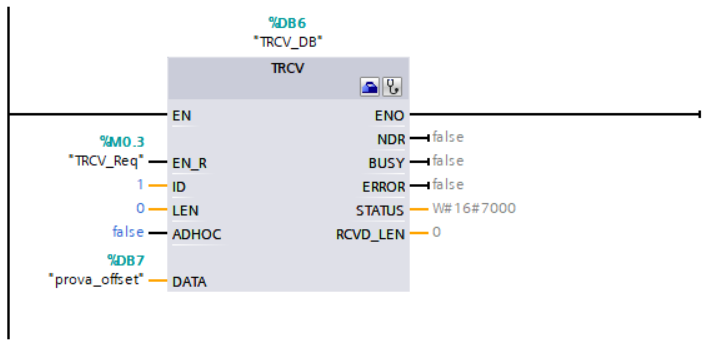
\includegraphics[width=0.8\linewidth]{capitolo3/figure/trcv.PNG}
    \caption{TRCV function the for TCP connection}
    \label{fig:trcv}
    \end{center}
    \end{figure}
\end{itemize}

\subsubsection{MATLAB}
To set up the TCP connection from MATLAB first of all a connection object has to be created. The tcpip function is offered from MATLAB to this purpose. It takes as parameters the IP address of the partner, i.e. the PLC, the connection port set up in the configuration phase in Tia Portal as second parameter. The third and the fourth are used to define the role of Matlab in the netwrok that will be created. In our case, being the master in the TCP communication, it will operate as a server.
The connection object is defined with the command written in Listing \ref{code1}

\begin{lstlisting}[style=htmlcssjs,caption={Creation of the connection object},label=code1]
t = tcpip('192.168.0.1', 2000, 'NetworkRole', 'server');
\end{lstlisting}




Matlab offers four functions to manage the connection:
\begin{itemize}
    \item \textbf{fopen()}. It opens the connection and requires the connection object as a parameter.
    \item \textbf{fclose()}. It closes the connection and requires the connection object as a parameter.
    \item \textbf{fwrite()}. It allows to send data from Matlab to the PLC through the previously established connection. It needs the connection object and the data that has to be sent as the two parameters.
    \item \textbf{fread()}. This function allows to read the data received through the connection. It has a required parameter, the connection object, and it is possible also to set the expected received data length as an optional parameter. It waits for the data and then return as output the read values when the expected length is reached or the connection timeout is expired.
\end{itemize}

\subsubsection{Data blocks}
Two data blocks were defined in Tia Portal:
\begin{itemize}
    \item Sent\_values, used to store the information about the actual position of the robot and send it to Matlab;
    \item Received\_values, used to store the information about the movements that the robot has to perform in order to reach a point or grab/release an object.
\end{itemize}
Both the data blocks have the same structure, defined as follows:
\begin{enumerate}
    \item Rotation, that stores an integer value corresponding to a certain counterclockwise rotation with respect to the initial position of the robot;
    \item Vertical, that stores an integer value corresponding to a certain vertical movement towards the base of the robot with respect to the initial position of the robot;
    \item Horizontal, that stores an integer value corresponding to a certain frontward movement with respect to the initial position of the robot;
    \item Gripper, that stores a boolean value that is true when the gripper of the robot is fully closed or has to be closed, while it is false when the gripper of the robot is fully open or has to be open. 
\end{enumerate}

\begin{figure*}[!h]
\centering
\subfloat[Sent\_values\label{fig:sent_values}]{
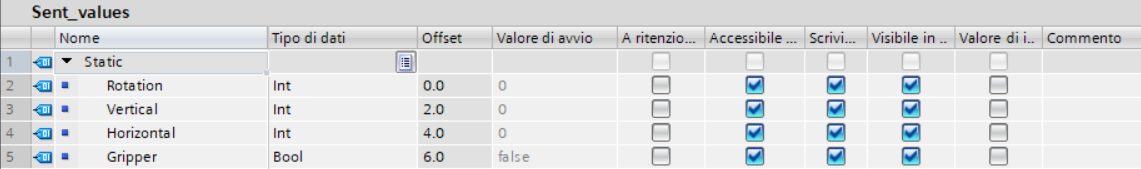
\includegraphics[width=1\linewidth]{capitolo3/figure/Sent_values.PNG}
}
\qquad
\subfloat[Received\_values\label{fig:received_values}]{
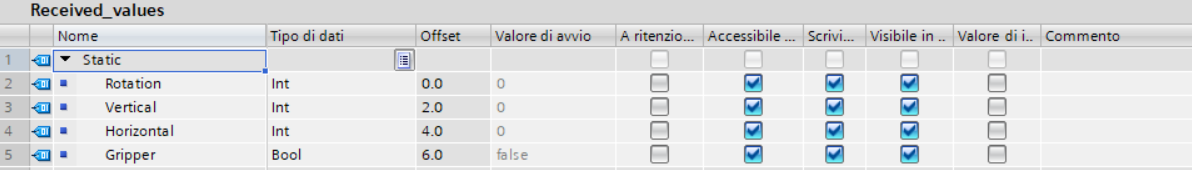
\includegraphics[width=1\linewidth]{capitolo3/figure/Received_values.PNG}
}
\caption{Data Blocks}
\label{fig:data_blocks}
\end{figure*}

\subsubsection{Matlab high level communication class, functions and scripts}
Some high level communication functions and scripts were written in Matlab in order to facilitate the PLC programming for a specific task.

The script \textit{Matlab\_PLC\_connection} creates a connection object and then open the connection listen for a client to connect. After the client connection, it initializes the \textit{old\_position} vector to the initial position of the robot.

\lstinputlisting[language=matlab,breaklines=true,caption={Matlab\_PLC\_connection.m}]{capitolo3/codes/Matlab_PLC_connection.m}

The script \textit{reset\_position} the connection buffer from remaining messages from the PLC and then reinitializes the vector \textit{old\_position} to the initial position of the robot. It is useful if the robot position is reset but the stop button has not been pressed, so the connection is still open.

\lstinputlisting[language=matlab,caption={reset\_position.m},breaklines=true]{capitolo3/codes/reset_position.m}

The function \textit{move\_robot()} was defined in order to move the robot: when the function is executed, it send a command to the PLC, that will move the robot, and then listen until the movement is completed and the PLC send back the position reached by the robot, which is written inside the \textit{old\_position} vector. If the robot is already in the desired position, the function terminates without doing nothing. The function has two required arguments:
\begin{itemize}
    \item connection, that is the connection object to use:
    \item old\_position, that is the old\_position vector used to store the position of the robot.
\end{itemize}
This function has also a series of couple of optional arguments. In particular they are:
\begin{itemize}
    \item the string 'rotation', followed by an integer which represent the a certain counterclockwise rotation with respect to the initial position of the robot. The initial position of the robot is associated with a value of $-5$ degrees since, when the robot is in the reset position it is not perfectly aligned with the perpendicular direction to the side of the basis. The limit switch is pressed when the position of the robotic arm coincide with $-5$ degrees.
    \item the string 'vertical', followed by an integer value corresponding to a certain vertical movement towards the base of the robot with respect to the initial position of the robot;
    \item the string 'horizontal', followed by an integer value corresponding to a certain frontward movement with respect to the initial position of the robot;
    \item the string 'gripper', followed by a boolean value that is true when the gripper of the robot is fully closed or has to be closed, while it is false when the gripper of the robot is fully open or has to be open. 
\end{itemize}

As it is possible to understand from the optional parameters definition, the positions that have to be passed are absolute positions with respect to the initial one.
If some of the optional parameters are not used, the will be set by default to the previous one.
The function returns the updated \textit{old\_position} vector, containing the reached position of the robot.

\lstinputlisting[language=matlab,caption={move\_robot.m},breaklines=true]{capitolo3/codes/move_robot.m}

The function \textit{emergency\_reset} closes the connection, resets the \textit{old\_position} vector and open again the connection. It has the connection as required argument and returns the reinitialized \textit{old\_position} vector.

\lstinputlisting[language=matlab,caption={emergency\_reset.m},breaklines=true]{capitolo3/codes/emergency_reset.m}

Futhermore it was defined the class \textit{gripper}, in order to make the use of the \textit{move\_robot} function more user-friendly. It has two properties:
\begin{itemize}
    \item open, that is equal to false;
    \item close, that is equal to true.
\end{itemize}

\lstinputlisting[language=matlab,caption={gripper.m},breaklines=true]{capitolo3/codes/gripper.m}


% Posizioni assolute: il valore che diamo da Matlab è il valore che deve raggiungere e non di quanto si deve spostare dalla sua posizione attuale

% mettere controllo lato matlab su valori negativi
% fino quando valore attuale è minore uguale di quello attuale

% Variables table
% Received_values:
% Rotation Int
% Vertical Int
% Horizontal Int 
% Gripper Bool (True -> Close; False -> Open)

%Matlab function move()
% optional arguments like 'rotation', value_rotation


\section{Ladder diagram}
\subsection{Variables table}
The following variables were defined in order to program the PLC:
\begin{enumerate}
    \item GripperOpenStop is a boolean that indicates that the gripper is fully open;
    \item GripperCounter is a boolean that is used to increment a counter that represents how much the gripper is open or closed;
    \item ArmBackStop is a boolean that indicates that the horizontal arm is completely set back;
    \item ArmHCounter is a boolean that is used to increment a counter that represents how much the horizontal arm is forward or backward;
    \item ArmTopStop is a boolean that indicates that the horizontal arm is completely set at the top;
    \item ArmRotationStop is a boolean that indicates that the robot is fully clockwise rotated;
    \item RotationalEncoder is an integer that indicates how much the robot is counterclockwise rotated and it is the output of an HSC (high speed counter);
    \item VerticalEncoder is an integer that indicates how much the horizontal arm is moved down (high speed counter);
    \item ConnectionButton is a boolean that is used to start the TCP connection with MATLAB;
    \item StopButton is a boolean that indicates that an emergency occurred and so the robot has to be stopped;
    \item ResetButton is a boolean that indicates that the robot position has to be reset to the initial one;
    \item In3 is a boolean that represents an unused input of the PLC (it was defined for possible future extension of this work);
    \item GripperOpen is a boolean that indicates that the gripper has to be open;
    \item GripperClose is a  boolean that indicates that the gripper has to be open;
    \item ArmFront is a boolean that indicates that the horizontal arm has to be moved forward;
    \item ArmBack is a boolean that indicates that the horizontal arm has to be moved back;
    \item ArmDown is a boolean that indicates that the horizontal arm has to be moved down;
    \item ArmUp is a boolean that indicates that the horizontal arm has to be moved up;
    \item RotationClockwise is a boolean that indicates that the robot has to be rotated clockwise;
    \item RotationCounterclockwise is a boolean that indicates that the robot has to be rotated counterclockwise;
    \item GreenLed is a boolean that indicates that the green LED must be switched on;
    \item RedLed is a boolean that indicates that the red LED must be switched on;
    \item System\_Byte is a byte that has to be activated from the properties of the PLC inside the clock and system merker tab (Figure\ref{fig:merker});
    \item FirstScan is the first bit of the system byte and it is a boolean that is set to True when the PLC is switched on, then it is immediately set to False;
    \item DiagStatusUpdate is the second bit of the system byte and it is not used in this project;
    \item AlwaysTRUE is the third bit of the system byte and it is a boolean always set to True;
    \item AlwaysFALSE is the fourth bit of the system byte and it is a boolean always set to False;
    \item RotationalCounter is an integer used to indicate how much the robot is rotated counterclockwise with respect to the initial position;
    \item Clock\_Byte is a byte representing the system clock and has to be activated from the properties of the PLC inside the clock and system merker tab (Figure\ref{fig:clock});
    \item Clock\_10Hz is the first  bit of the clock byte and it is set to True and immediately set to False at the frequency of 10 Hz;
    \item Clock\_5Hz is the second bit of the clock byte and it is set to True and immediately set to False at the frequency of 5 Hz;
    \item Clock\_2.5Hz is the third  bit of the clock byte and it is set to True and immediately set to False at the frequency of 2.5 Hz;
    \item Clock\_2Hz is the fourth  bit of the clock byte and it is set to True and immediately set to False at the frequency of 2 Hz;
    \item Clock\_1.25Hz is the fifth  bit of the clock byte and it is set to True and immediately set to False at the frequency of 1.25 Hz;
    \item Clock\_1Hz is the sixth bit of the clock byte and it is set to True and immediately set to False at the frequency of 1 Hz;
    \item Clock\_0.625Hz is the seventh bit of the clock byte and it is set to True and immediately set to False at the frequency of 0.625 Hz;
    \item Clock\_0.5Hz is the eighth bit of the clock byte and it is set to True and immediately set to False at the frequency of 0.5 Hz;
    \item VerticalCounter is an integer used to indicate how much the horizontal arm is moved down with respect to the initial position;
    \item ForceReset is a boolean that is set to True during the reset of the robot to the initial position;
    \item ResetCompleted is a boolean that is set to True when the reset operation is completed;
    \item TCON\_Req is a boolean that was used during the environment setup phase to establish the TCP connection with MATLAB;
    \item TDIS\_Req is a boolean that was used during the environment setup phase to close the TCP connection with MATLAB;
    \item TSEND\_Req is a boolean that was used during the environment setup phase to write inside the TCP connection send buffer;
    \item TRCV\_Req is a boolean that was used during the environment setup phase to read the TCP connection receive buffer;
    \item VerticalOverCounter is an integer that represents the maximum of the confidence interval for the vertical movement;
    \item VerticalUnderCounter is an integer  that represents the minimum  of the confidence interval for the vertical movement;
    \item RotationOverCounter is an integer that represents the maximum of the confidence interval for the rotation movement;
    \item RotationUnderCounter is an integer that represents the minimum  of the confidence interval for the rotation movement;
    \item NormalizedRotationUnderCounter is an integer that is equal to the RotationUnderCounter value, with the exception that, when RotationUnderCounter is negative, it is zero;
    \item NormalizedVerticalUnderCounter is an integer that is equal to the VerticalUnderCounter value, with the exception that, when VerticalUnderCounter is negative, it is zero;
    \item StopAll is a boolean that is True when the emergency stop button is pressed;
    \item HRegistered is a boolean that indicates that the horizontal position of the robot has been written into the Sent\_values data block;
    \item VRegistered is a boolean that indicates that the vertical position of the robot has been written into the Sent\_values data block;
    \item RRegistered is a boolean that indicates that the rotational position of the robot has been written into the Sent\_values data block.
\end{enumerate}

\begin{figure*}[!h]
\centering
\subfloat[Variables table (1)\label{fig:variables_table1}]{
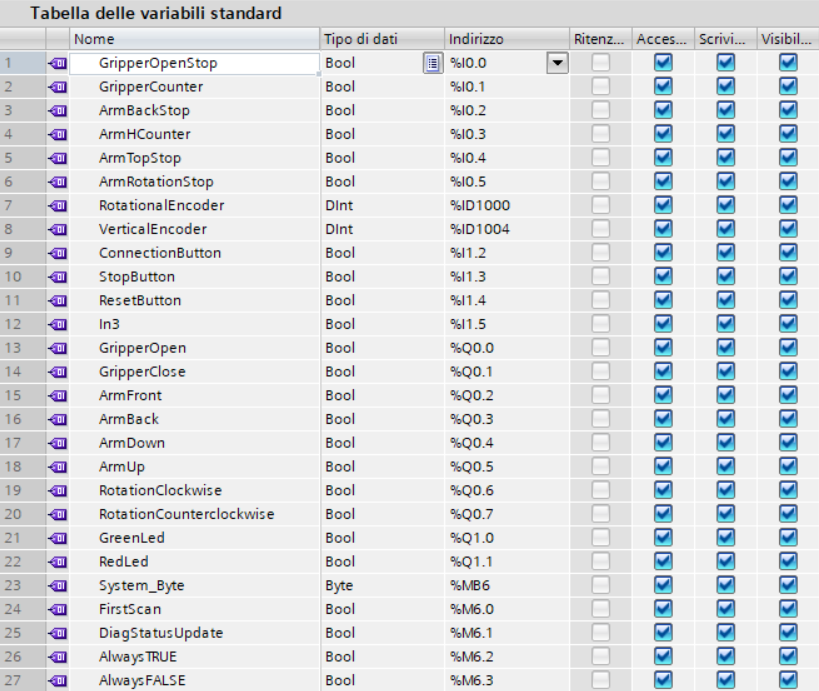
\includegraphics[width=0.8\linewidth]{capitolo3/figure/tabella_variabili1.PNG}
}
\qquad
\subfloat[Variables table (2)\label{fig:variables_table2}]{
\includegraphics[width=0.8\linewidth]{capitolo3/figure/tabella_variabili2.PNG}
}
\caption{Variables table}
\label{variables_table}
\end{figure*}

\begin{figure}[!h]
\begin{center}
\includegraphics[width=0.6\linewidth]{capitolo3/figure/system_merker_byte_activation.PNG}
\caption{System byte activation }
\label{fig:merker}
\end{center}
\end{figure}

\begin{figure}[!h]
\begin{center}
\includegraphics[width=0.6\linewidth]{capitolo3/figure/Clock_merker_activation.PNG}
\caption{Clock merkers activation}
\label{fig:clock}
\end{center}
\end{figure}

\newpage
\subsection{Ladder diagram}
\label{sec:ladder}
The first operation performed when the PLC is turned on is the reset of the robot to its reference initial position.
\begin{figure}[!h]
\begin{center}
\includegraphics[width=0.6\linewidth]{capitolo3/figure/Reset.png}
\caption{Position initialization}
\label{fig:reset}
\end{center}
\end{figure}


As it is possible to see in Figure\ref{fig:reset}, the ForceReset variable is set to True on the startup and then it is self-retained until the reset operation is completed (when the ResetCompleted variable is set to True).

\begin{figure}[!h]
\begin{center}
\includegraphics[width=0.6\linewidth]{capitolo3/figure/Segmento1_18.PNG}
\caption{Reset completed}
\label{fig:reset_completed}
\end{center}
\end{figure}

The ResetCompleted variable is set when all the limit switches are pressed (Figure\ref{fig:reset_completed}).

\begin{figure}[!h]
\begin{center}
\includegraphics[width=0.6\linewidth]{capitolo3/figure/reset_button.PNG}
\caption{Reset button}
\label{fig:reset_button}
\end{center}
\end{figure}

When the reset button is pressed and hold for 2 seconds, the force reset variable is set and than it is self-retained until the reset is completed (Figure\ref{fig:reset_button}).


\begin{figure}[!h]
\begin{center}
\includegraphics[width=0.6\linewidth]{capitolo3/figure/Segmento1_1_GO.PNG}
\caption{Gripper open}
\label{fig:gripper_open}
\end{center}
\end{figure}

As it is possible  to see in Figure\ref{fig:gripper_open}, the gripper is open when the corresponding value received from MATLAB is False or during the reset operation. The movement continues until the corresponding limit switch is pressed or the emergency stop is activated. During the opening of the gripper TSEND\_Req is reset because it has to be set when all the movements are completed.


\begin{figure}[!h]
\begin{center}
\includegraphics[width=0.6\linewidth]{capitolo3/figure/Segmento1_2_GC.PNG}
\caption{Gripper close}
\label{fig:gripper_close}
\end{center}
\end{figure}

As it is possible  to see in Figure\ref{fig:gripper_close}, the gripper is closed when the corresponding value received from MATLAB is True and the emergency stop has not been activated. The movement continues until the motor is forced three times. During the closing of the gripper TSEND\_Req is reset because it has to be set when all the movements are completed.

\begin{figure}[!h]
\begin{center}
\includegraphics[width=0.6\linewidth]{capitolo3/figure/Segmento1_9.PNG}
\caption{Gripper counter}
\label{fig:gripper_counter}
\end{center}
\end{figure}

As it is possible  to see in Figure\ref{fig:gripper_counter}, the gripper counter is increased during the closure of the gripper with a clock of 10 Hz, which corresponds to the gripper pulse counter frequency. The gripper counter is decreased each time the gripper pulse counter is set during the closure of the gripper. In this way, it is increased and decreased simultaneously. However, if the motor is forced and thus the pulse counter is not switched on, the gripper counter is only increased. The gripper counter is reset when the gripper is opening or when the corresponding limit switch is pressed.

\begin{figure}[!h]
\begin{center}
\includegraphics[width=0.6\linewidth]{capitolo3/figure/Segmento1_16.PNG}
\caption{Gripper status}
\label{fig:gripper_status}
\end{center}
\end{figure}

As it is possible to see in Figure\ref{fig:gripper_status}, the gripper status counter is increased during the opening of the gripper each time the gripper pulse counter is set. The gripper status counter is decreased during the closure of the gripper each time the gripper pulse counter is set. In this way, it is possible to store the information how the gripper is open or closed. The gripper status counter is reset when the corresponding limit switch is pressed.

\begin{figure}[!h]
\begin{center}
\includegraphics[width=0.6\linewidth]{capitolo3/figure/Segmento1_4_AB.PNG}
\caption{Arm back}
\label{fig:arm_back}
\end{center}
\end{figure}

As it is possible  to see in Figure\ref{fig:arm_back}, the horizontal arm of the robot is moved backward when the corresponding value received from MATLAB is less than the ArmHStatus counter value or during the reset operation. In both cases the movement is stopped if the emergency stop is activated of if the corresponding limit switch is pressed. During the movement of the arm TSEND\_Req is reset because it has to be set when all the movements are completed.


\begin{figure}[!h]
\begin{center}
\includegraphics[width=0.6\linewidth]{capitolo3/figure/Segmento1_3_AF.PNG}
\caption{Arm front}
\label{fig:arm_front}
\end{center}
\end{figure}

As it is possible  to see in Figure\ref{fig:arm_front}, the horizontal arm of the robot is moved forward when the corresponding value received from MATLAB is greater than ArmHStatus counter value and the emergency stop has not been activated. The movement is stopped if the motor is forced three times. During the movement of the arm TSEND\_Req is reset because it has to be set when all the movements are completed.

\begin{figure}[!h]
\begin{center}
\includegraphics[width=0.6\linewidth]{capitolo3/figure/Segmento1_10.PNG}
\caption{Arm horizontal movement counter}
\label{fig:arm_h_counter}
\end{center}
\end{figure}

As it is possible  to see in Figure\ref{fig:arm_h_counter}, the horizontal movement counter is increased during the forward movement of the horizontal arm with a clock of 10 Hz, which corresponds to the corresponding pulse counter frequency. The horizontal  movement counter is decreased each time the corresponding pulse counter is set during the forward movement. In this way, it is increased and decreased simultaneously. However, if the motor is forced and thus the pulse counter is not switched on, the horizontal movement counter is only increased. The horizontal movement counter is reset during the backward movement or when the corresponding limit switch is pressed.

\begin{figure}[!h]
\begin{center}
\includegraphics[width=0.6\linewidth]{capitolo3/figure/Segmento1_11.PNG}
\caption{Arm horizontal movement status}
\label{fig:arm_h_status}
\end{center}
\end{figure}

As it is possible to see in Figure\ref{fig:arm_h_status}, the arm horizontal movement status counter is increased during the forward movement each time the corresponding pulse counter is set. The arm horizontal movement status counter is decreased during the backward movement each time the corresponding pulse counter is set. In this way, it is possible to store the information about the horizontal position of the arm. The arm is reset when the corresponding limit switch is pressed.

\begin{figure}[!h]
\begin{center}
\includegraphics[width=0.8\linewidth]{capitolo3/figure/hsc_conf.PNG}
\caption{HSC activation and configuration}
\label{fig:hsc_config}
\end{center}
\end{figure}

The vertical and rotational movements are monitored using the two encoders. Two HSCs (high speed counters) were activated to read values from the encoder from the PLC properties inside the HSC tab and were set to A/B count mode (Figure\ref{fig:hsc_config}). In this way the HSCs value is incremented or decremented by 1 depending on the time order of the rising edges of the corresponding encoder signals (A and B).

\begin{figure*}[!h]
\centering
\subfloat[Horizontal encoder addresses\label{fig:h_encoder_addresses}]{
\includegraphics[width=0.5\linewidth]{capitolo3/figure/horizontal_encoder.PNG}
}
\qquad
\subfloat[Vertical encoder addresses\label{fig:v_encoder_addresses}]{
\includegraphics[width=0.5\linewidth]{capitolo3/figure/vertical_encoder.PNG}
}
\caption{HSCs values addresses configuration}
\label{fig:encoder_addresses}
\end{figure*}

The rotational and vertical HSCs were configured to store the counter valued respectively in the memory addresses of the variables RotationalEncoder and VerticalEncoder (Figure\ref{fig:encoder_addresses}). 

The input frequency for the HSC was set to 2.5 kHz (Figure \ref{fig:encoder_frequency}), because the maximum freuqency of the encoders is 1 kHz and accordingly to the Nyquist theorem the sampling frequency should be greater or equal to the double of the maximum frequency of the signal. 

\begin{figure}[!h]
\centering
\caption{Encoders frequency}\label{fig:encoder_frequency}]{
\includegraphics[width=0.8\linewidth]{capitolo3/figure/freq_HSC.PNG}
}

\end{figure}

\begin{figure*}[!h]
\centering
\subfloat[HSC 1\label{fig:hsc1}]{
\includegraphics[width=0.4\linewidth]{capitolo3/figure/Segmento1_14.PNG}
}
\qquad
\subfloat[HSC 2\label{fig:hsc2}]{
\includegraphics[width=0.4\linewidth]{capitolo3/figure/Segmento1_15.PNG}
}
\caption{HSCs}
\label{fig:HSC}
\end{figure*}

The rotation HSC (Figure\ref{fig:hsc1}) and the vertical movement HSC (Figure\ref{fig:hsc2}) are stopped when the corresponding limit switch is pressed.

\begin{figure*}[!h]
\centering
\subfloat[RotationalEncoder variable copy\label{fig:rotational_encoder_copy}]{
\includegraphics[width=0.6\linewidth]{capitolo3/figure/Segmento1_12.PNG}
}
\qquad
\subfloat[VerticalEncoder variable copy\label{fig:vertical_encoder_copy}]{
\includegraphics[width=0.6\linewidth]{capitolo3/figure/Segmento1_13.PNG}
}
\caption{HSCs variables copy}
\label{fig:encoder_copy}
\end{figure*}

The values stored in the variables corresponding to the two HSCs values were copied inside the variables RotationalCounter and VerticalCounter (Figure\ref{fig:encoder_copy}). This was done because it is a good practice to avoid to use directly the variables in which the values counted by the HSCs are stored: in fact in this way it is impossible that those values are erroneously modified.

\begin{figure*}[!h]
\centering
\subfloat[Rotation confidence interval\label{fig:rotational_confidence_interval}]{
\includegraphics[width=0.4\linewidth]{capitolo3/figure/Segmento1_20.PNG}
}
\qquad
\subfloat[Vertical confidence interval\label{fig:vertical_confidence_interval}]{
\includegraphics[width=0.4\linewidth]{capitolo3/figure/Segmento1_19.PNG}
}
\caption{Confidence intervals}
\label{fig:confidence_intervals}
\end{figure*}

The increment on subsequent values that were possible to read from the encoders was not equal to 1 unit. Therefore they were defined two confidence intervals (one for each encoder), within which the position error is negligible (in fact the difference cannot be noticed by a human eye). The intervals are 20 units large and are centered in the corresponding desired positions. The maximum and the minimum of each interval computation is shown in Figure\ref{fig:confidence_intervals}.

\begin{figure}[!h]
\begin{center}
\includegraphics[width=0.5\linewidth]{capitolo3/figure/Segmento1_21.PNG}
\caption{Confidence intervals minimum adjustment}
\label{fig:confidence_min}
\end{center}
\end{figure}

It may happen that the minimum of the confidence intervals is a negative value. When this happens, the minimum is set to 0 by using two MAX blocks in which each of the computed minimums are compared with 0 and the maximum between the compared values is then stored in a new variable called NormalizedRotationUnderCounter for the rotation and NormalizedVerticalUnderCounter for the vertical movement (Figure\ref{fig:confidence_min}). 


\begin{figure}[!h]
\begin{center}
\includegraphics[width=0.6\linewidth]{capitolo3/figure/Segmento1_6_AU.PNG}
\caption{Arm up}
\label{fig:arm_up}
\end{center}
\end{figure}

As it is possible  to see in Figure\ref{fig:arm_up}, the horizontal arm of the robot is moved up when the minimum of the corresponding confidence interval is less than the value read from the corresponding encoder or during the reset operation. In both cases  the movement continues until the corresponding limit switch is pressed or the emergency stop is activated. During the movement of the arm TSEND\_Req is reset because it has to be set when all the movements are completed.


\begin{figure}[!h]
\begin{center}
\includegraphics[width=0.6\linewidth]{capitolo3/figure/Segmento1_5_AD.PNG}
\caption{Arm down}
\label{fig:arm_down}
\end{center}
\end{figure}

As it is possible  to see in Figure\ref{fig:arm_down}, the horizontal arm of the robot is moved down when the maximum of the corresponding confidence interval is greater than the value read from the corresponding encoder. The movement is stopped if the emergency stop is activated or the maximum reachable point is reached. During the movement of the arm TSEND\_Req is reset because it has to be set when all the movements are completed.


\begin{figure}[!h]
\begin{center}
\includegraphics[width=0.6\linewidth]{capitolo3/figure/Segmento1_7_RC.PNG}
\caption{Rotation clockwise}
\label{fig:rotation_clockwise}
\end{center}
\end{figure}

As it is possible  to see in Figure\ref{fig:rotation_clockwise}, the robot is rotated clockwise when the maximum of the corresponding confidence interval is less than the value read from the corresponding encoder or during the reset operation. In both cases  the movement continues until the corresponding limit switch is pressed or the emergency stop is activated. During the rotation of the robot TSEND\_Req is reset because it has to be set when all the movements are completed.


\begin{figure}[!h]
\begin{center}
\includegraphics[width=0.6\linewidth]{capitolo3/figure/Segmento1_8_RCC.PNG}
\caption{Rotation counterclockwise}
\label{fig:rotation_counterclockwise}
\end{center}
\end{figure}

As it is possible  to see in Figure\ref{fig:rotation_counterclockwise}, the robot is rotated counterclockwise when the minimum of the corresponding confidence interval is greater than the value read from the corresponding encoder. The movement is stopped if the emergency stop is activated or the maximum reachable point is reached. During the rotation TSEND\_Req is reset because it has to be set when all the movements are completed.

\begin{figure*}[!h]
\centering
\subfloat[Horizontal value update in Sent\_values\label{fig:hregistered}]{
\includegraphics[width=0.8\linewidth]{capitolo3/figure/Segmento1_25.PNG}
}
\qquad
\subfloat[Vertical value update in Sent\_values\label{fig:vregistered}]{
\includegraphics[width=0.8\linewidth]{capitolo3/figure/Segmento1_26.PNG}
}
\qquad
\subfloat[Rotation value update in Sent\_values\label{fig:rregistered}]{
\includegraphics[width=0.8\linewidth]{capitolo3/figure/Segmento1_27.PNG}
}
\qquad
\subfloat[Gripper value update in Sent\_values\label{fig:rregistered}]{
\includegraphics[width=0.8\linewidth]{capitolo3/figure/gripper_registered.PNG}
}
\caption{Sent\_values update}
\label{fig:sent_update}
\end{figure*}

As it is possible to see in Figure\ref{fig:sent_update} the values of the variables stored into the Sent\_values data block are updated each time the corresponding movement has ended.

\begin{figure}[!h]
\begin{center}
\includegraphics[width=0.8\linewidth]{capitolo3/figure/send.PNG}
\caption{Send values to MATLAB}
\label{fig:send}
\end{center}
\end{figure}

As it is possible to see in Figure\ref{fig:send}, when all the movements are completed and the corresponding reached position has been written into the Sent\_values data block, after one second (the delay ensure that the write operations are finished before to send the data), TSEND\_Req is set and thus these values are sent to MATLAB. 

\begin{figure*}[!h]
\centering
\subfloat[Connection block\label{fig:connection_block}]{
\includegraphics[width=0.5\linewidth]{capitolo3/figure/Segmento2.PNG}
}
\qquad
\subfloat[Disconnection block\label{fig:disconnection_block}]{
\includegraphics[width=0.5\linewidth]{capitolo3/figure/Segmento3.PNG}
}
\qquad
\subfloat[Send block\label{fig:send_block}]{
\includegraphics[width=0.5\linewidth]{capitolo3/figure/Segmento4.PNG}
}
\qquad
\subfloat[Receive block\label{fig:receive_block}]{
\includegraphics[width=0.5\linewidth]{capitolo3/figure/Segmento5.PNG}
}
\caption{TCP Connection blocks}
\label{fig:segments_2_3_4_5}
\end{figure*}

As it is possible to see in Figure\ref{fig:connection_block} the PLC connection with Matlab is open on the PLC side when the connection button is pressed.
From Figure\ref{fig:disconnection_block} it is possible to see that when the emergency stop button is pressed the connection is closed on the PLC side.
As it is possible to see in Figure\ref{fig:send_block}, when TSEND\_Req is set, the values stored in Sent\_values data block are sent to Matlab.
From Figure\ref{fig:receive_block} it is possible to see that the Matlab and those values are then stored into the Received\_values data block.

\begin{figure}[!h]
\begin{center}
\includegraphics[width=0.8\linewidth]{capitolo3/figure/stop_button.PNG}
\caption{Stop button}
\label{fig:stop_button}
\end{center}
\end{figure}

As it is possible to see in Figure\ref{fig:stop_button}, when the stop button is pressed, the emergency stop is activated and then it is self-retained.

\begin{figure}[!h]
\begin{center}
\includegraphics[width=0.8\linewidth]{capitolo3/figure/stop_reset.PNG}
\caption{Emergency stop during reset}
\label{fig:stop_reset}
\end{center}
\end{figure}

As it is possible to see in Figure\ref{fig:stop_reset}, the pressure of the emergency stop button reset the ForceReset variable, thus it is possible to stop the robot also during the reset operation.

\begin{figure}[!h]
\begin{center}
\includegraphics[width=0.8\linewidth]{capitolo3/figure/red_led_stop.PNG}
\caption{Red LED}
\label{fig:red_led}
\end{center}
\end{figure}

As it is possible to see in Figure\ref{fig:red_led}, when the emergency stop is active the red LED is switched on, while during the reset operation it blinks with a frequency of 1Hz.

\begin{figure}[!h]
\begin{center}
\includegraphics[width=0.6\linewidth]{capitolo3/figure/green_led.PNG}
\caption{Green LED}
\label{fig:green_led}
\end{center}
\end{figure}

As it is possible to see in Figure\ref{fig:green_led}, the green LED is switched on when the robot is not moving and it has not been stopped using the emergency stop button, while it blinks when the robot is moving.

\begin{figure}[!h]
\begin{center}
\includegraphics[width=0.4\linewidth]{capitolo3/figure/reset_operations.PNG}
\caption{Reset operations}
\label{fig:reset_operations}
\end{center}
\end{figure}

As it is possible to see in Figure\ref{fig:reset_operations}, during the reset operation all the variables inside the Sent\_values and Received\_values data blocks are imposed equal to 0 or false depending on their type (integer or boolean), the emergency stop is reset and the green LED is switched off until the reset operation is completed.

\newpage
\section{CoppeliaSim model}

The model of the robotic arm has been created through the version 4.1.0 of the software CoppeliaSim (formerly known as \textit{V-REP}). 
The goal of the model realization process is to create a environment which is able to perform simulations of the works that will be done by the robot. The approach of the simulations enable the project developers to test in a secure sandbox all the movement which the robot needs to perform, and allow (if it is well designed) to understand which are the constraints in the moves during the scene performance.
To accomplish this task, the model was realized in order to work in two different ways:
\begin{itemize}
    \item a simulation in which the robot can reach all the points through \textbf{direct} kinematics, in which the movements are imposed by passing the values to set for each joint;
    \item a simulation in which the robot can reach all the points through \textbf{inverse} kinematics, in which the movements are imposed by passing directly the point the robot's tip need to reach.
\end{itemize}
The process of modeling the robot requires an analysis of the pieces which need to be realized in the model in order to reach a good level of approximation. 

In this specific project, the model, which is represented in Figure \ref{fig:model_robot_image}, is composed by two main elements which represent the base on which the robot lies and the robot itself. Moreover, on the base element, all the electronic components which enable motors and sensors are modeled to represent obstacles for the arm movements, while on the robot components, all the joins, links and support structures are implemented.

\begin{figure*}[h]
\centering
\subfloat[Real Robot\label{fig:real_robot_image}]{
\includegraphics[width=0.45\linewidth]{capitolo3/figure/3D-Robot-24V}
}
\qquad
\subfloat[3D Model\label{fig:model_robot_image}]{
\includegraphics[width=0.45\linewidth]{capitolo3/figure/3Dmodel}
}
\caption{Comparative between real robot and 3D model}
\label{comparative_models}
\end{figure*}

No 3D model was provided by the manufacturer of the robot and, in particular, on the website of the \textit{Fischertecnick robotic arm}\cite{3DRobot291:online}, only a series of images, videos and datasheets are provided.
For this reason, not having a complete drawing of the robot with quotas and measures, a meticulous process of measurement was necessary and it strictly followed the one of modeling.
All the elements inside the model are realized by only using a set of primitive shapes (i.e., cuboids and cylinders), joints (i.e., revolute and prismatic ones) and sensors (the proximity ones). 
More in details, all the moving parts of the robot with except of the gripper (which is a static part), are realized as moving part of the 3D model.
With regard to the gripper instead, it could be implemented a new version which enable the grip ability in future works. Inspecting the model one revolute joint (which enable the robot to rotate) and two prismatic joints (one which enable the robot to move vertically and the other one for the horizontal movements) can be found. As for the physics linked to the real model, each movement for the 3D model robot has a spatial range:

\begin{itemize}
    \item the revolute joint can assume position in the interval $\interval{-5.00}{330.00}$, with a range of 335\degree;
    \item the prismatic joint for vertical movements can assume position in the interval  $\interval{-14.00}{0.00}$, with a range of \SI{14.00}{\centi\metre};
    \item the prismatic joint for horizontal movements can assume position in the interval  $\interval{0.00}{9.50}$, with a range of \SI{9.50}{\centi\metre}.
\end{itemize}

More specifically, to better simulate the real behaviour of the robot, all the \textit{end-of-stroke} buttons are implemented through proximity sensors whose, linked to a \textit{Non threaded} child script, enable the robot to stop exactly when the end-of-stroke buttons would be pressed in real world. In the used proximity sensors, which are of type \textit{ultrasonic}, the property ``Explicit handling" is enabled (to allow the control through the script), the used ``Volume parameters" are listed in , as shown in Figure \ref{fig:volume_parameters}.

\begin{figure}[h]
\begin{center}
\includegraphics[width=0.5\linewidth]{capitolo3/figure/volume_parameters}
\caption{Volume parameters}
\label{fig:volume_parameters} 
\end{center}
\end{figure}

The sensors are enabled on both side of each link which can be moved and they are ``sensitive" only to the particular joint that will be able to approach them. To accomplish this specific task, all the links, which have to be sensed by the sensors, have to be configured as \textbf{Detectable} objects, as shown in Figure \ref{fig:detectable_objects}.

\begin{figure*}[h]
\centering
\subfloat[Detectable object\label{fig:detectable_objects}]{
\includegraphics[width=0.45\linewidth]{capitolo3/figure/detectable_objects}
}
\qquad
\subfloat[Collidable object\label{fig:collidable_object}]{
\includegraphics[width=0.45\linewidth]{capitolo3/figure/collidable_object}
}
\caption{Setup for object}
\label{collision_setup}
\end{figure*}

Furthermore, in the realized scene, it is also configured a system to detect collision. More specifically, a collection is configured which contains all the ``moving elements" of the robot, as shown in the Figure \ref{fig:robot_collection}. It is also needed to add a new object collision in the ``Calculation Modules" window as shown in Figure \ref{fig:model_robot_image}, reached from the voice ``Tools" in the menubar. Next step requires to set all the elements which can collide. To do that, object needs to be a ``Collidable Object", as shown in Figure \ref{fig:collidable_object}.

\begin{figure*}[h!]
\centering
\subfloat[Robot collection\label{fig:robot_collection}]{
\includegraphics[width=0.45\linewidth]{capitolo3/figure/robot_collection}
}
\qquad
\subfloat[Calculation modules\label{fig:model_robot_image}]{
\includegraphics[width=0.45\linewidth]{capitolo3/figure/calculation_modules}
}
\caption{Setup for collision}
\label{collision_setup}
\end{figure*}

Listing \ref{lst:non_threaded_collision} display the lua code used to manage the sensors and the collisions. 

In particular the content of the \textit{sysCall\_init()} is used to retrieve the handle for the object which are used in the other functions. In the \textit{sysCall\_actuation()} the code is written to make movements up to when the joints are not pressing the end-of-stroke buttons. Inside the \textit{sysCall\_sensing()} collision checks are done and sensing is performed through the sensors.

\lstinputlisting[language=lua,breaklines=true,caption={Non threaded child script for register collision},label={lst:non_threaded_collision}]{capitolo3/codes/non-threaded-collision.lua}

Thanks to this kind of implementation, the 3D simulations run on CoppeliaSim allow the designers to understand the real robotic arm limits before to act on it. For example, the simulation can be used to understand if a movement can be dangerous for the robot, or it can be used to understand how a movement can be performed (by moving one joint at a time, or more than one).

%First we added the fixed base from the "Add" menu, clicking on "Primitive shape" an then on "Cuboid". In the following window, the dimensions of the base of the Fischertecnick robotic arm has to be set. They are $25.5 \mathr{cm~x}~18.5 \mathr{cm~x}~2cm (width ~x~ depth ~x~ height)$. Then, the first link can be added selecting "Primitive shape -> Cylinder". The diameter is equal to $9\mathr{~cm}$, the height, considering also the distance of the rotation gear from the base and its thickness, is $2.5\mathr{~cm}$. To place the link in the correct position, click on "Object/item shift" in the navbar and then select the cylinder. In "Position" tab select the reference system for the shifting and then set the desired values. The robotic arm is centered with respect to the Y-axis, whereas for the X-axis it is placed so that the border of the cylinder coincide with the one of the base.
%\begin{figure}[!h]
%\begin{center}
%\includegraphics[width=\linewidth]{capitolo3/figure/shifting_component.png}
%\caption{Shifting a component}
%\label{fig:trcv}
%\end{center}
%\end{figure}

%The next step is to add the revolute joint so that the cylinder can turn around itself. Click on "Add -> Joint -> Revolute". Then move it in the correct position, as done for the cylinder, and set the hierarchy as in Figure\ref{fig:first_hierarchy} to have the correct dependency.
%\begin{figure}[!h]
%\begin{center}
%\includegraphics[width=\linewidth]{capitolo3/figure/hierarchy1.png}
%\caption{Setting the hierarchy}
%\label{fig:first_hierarchy} 
%\end{center}
%\end{figure}

%The vertical link will be created utilizing a cuboid with dimensions equal to $6 cm x 6 cm x 19cm (width x depth x height)$. A prismatic joint is then added between the first link and this second link.

\section{Inverse Kinematic}
% COPIATO
The inverse kinematics problem consists of the determination of the joint variables corresponding to a given end-effector position and orientation. The solution to this problem is of fundamental importance in order to transform the motion specifications, assigned to the end-effector in the operational space, into the corresponding joint space motions that allow execution of the desired motion.

\begin{figure}[h]
\begin{center}
\includegraphics[width=0.75\linewidth]{capitolo3/figure/ik}
\caption{Inverse Kinematic and Direct Kinematic}
\label{fig:ik} 
\end{center}
\end{figure}

Generally the aim is to find a robot configuration $q$ such that $\varphi(q)=y*$.
If and only if $\varphi$ is invertible $q* = \varphi^{-1}(y*)$.
But in general, $\varphi$ will not be invertible:
\begin{itemize}
    \item The pre-image $\varphi^{-1}(y*)$ may be empty: no configuration can generate the desired $y*$;
    \item The pre-image $\varphi^{-1}(y*)$ may be large: many configurations can generate the desired $y*$.
\end{itemize}

The inverse kinematics problem is very complex for the following reasons:
\begin{itemize}
    \item it is not always possible to find a closed form solution, in fact the equations to solve are in general nonlinear;
    \item multiple (depending on the number of degrees of freedom and on the number of non null DH parameters) or infinite (in the case of a kinematically redundant manipulator) solutions may exist;
    \item there might be no solution, in fact the existence of a solution is guaranteed only if the point belongs to the manipulator dexterous workspace;
    \item it is not always possible to compute all the admissible solutions (depending on the solution technique applied).
\end{itemize}

The solutions can be of two kind:
\begin{itemize}
    \item analytical (in closed form);
    \item numerical.
\end{itemize}

The analytical solutions can be:
\begin{itemize}
    \item geometric inspection;
    \item algebric methods.
\end{itemize}

The numerical solutions methods are needed if the manipulator is redundant or if the closed form solution is not available. They use the Jacobian matrix of the direct kinematic map and two different iterative methods can be followed:
\begin{itemize}
    \item the Newton method;
    \item the gradient method.
\end{itemize}

In the Newton method it is important that the Jacobian matrix of the direct kinematic map is not singular, because it has to be inverted in order to compute the inverse kinematic (in the case of robot redundancy the pseudo inverse matrix is used).

The gradient method is based on the iterative computation of the derivative of the error (the objective is to minimize a certain cost function) and on the integration with respect to the initial conditions. It is important to choose a multiplicative factor $\alpha$, called step size, such that the error function decreases at each iteration. It has to be greater than 0, but also not too much great in order to avoid to "miss" the minimum of the function.

%Parte di CoppeliaSim
\subsection{Inverse Kinematic in CoppeliaSim}
Another important usage of CoppeliaSim is for resolving the inverse kinematic. More specifically, given a particular robot model well configured, the simulator is able to make the tip of the robot reach the minimum distance to a specific point in the space (i.e., if the point is inside the workspace of the robot, it is directly reached, so the minimum distance between tip and target point will be zero, else the robot is oriented and moved in order to have the minimum distance between the tip and the target point, but it will be greater than zero).

As already discussed, the inverse kinematic analysis is really useful when it is needed to perform a particular action, due to the fact that starting by a particular point in the \textit{3D space}, it is possible to retrive the same point (if it is inside the workspace) in the \textit{joint space}. This possibility enable the designers to realize particular scenes in which the robot can perform actions which makes it interact with the surrounding environment (i.e., ambience and objects).

\begin{figure}[h]
\begin{center}
\includegraphics[width=0.75\linewidth]{capitolo3/figure/demo_ik}
\caption{Demo starting position in scene for Inverse Kinematic}
\label{fig:demo_ik} 
\end{center}
\end{figure}

In the case of this project, the presented demo consists of moving an object between two different positions. More specifically, the initial scene of the demo is depicted in Figure \ref{fig:demo_ik}. Here the robot is able to move from its reset position to the one which allow it to pick up a cylinder in position \textbf{A} and move it to position \textbf{B}. In the end the robot returns in its reset position.
The demo is also able to repeat these movements indefinitely up to when a user stops it.

To set the demo on CoppeliaSim, a path was created, in which the five points are located where the tip of the robot should be for performing a specific action (i.e., prepare to pick the cylinder, pick it, move it, release it). Two \textit{dummy} elements are created, one for the tip, which are moved inside the center of the gripper, and one for the target, which is the point the robot needs to follow.

In order to move from direct kinematic to inverse kinematic, it is needed\cite{VrepCopp83:online} to change the mode for all the joint in the robot, from \textit{Torque/force mode} to \textit{Inverse kinematics mode}.

To enable the target to follow the path\cite{PathFoll72:online}, a \texit{threaded child script}, is attached to the target dummy element. Its code can be read in the Listing \ref{lst:path_pick_release} and uses the function ``followPath" to make the target point follow the five-points path already described.

\lstinputlisting[language=lua,breaklines=true,caption={Threaded child script for follow the path},label={lst:path_pick_release}]{capitolo3/codes/follow_path.lua}

By doing so, it is possible, by only running the simulation, to see if the robot will collide with any object during the execution of the demo and to adjust the trajectory of the points. More important, thanks to the inverse kinematics resolution from CoppeliaSim, it is also possible to retrieve the values for the \textit{joint space} and to use them to manage the real robot to perform the same demo in the real world.

\begin{figure}[h]
\begin{center}
\includegraphics[width=\linewidth]{capitolo3/figure/print_distance}
\caption{Simulation of the demo and debug of the point position in the joint space}
\label{fig:print_distance} 
\end{center}
\end{figure}

To simplify these operation of reading the joint variables from the simulator, a \textit{non threaded child script} is realized and attached to the first element of the robot which prints the point position in the joint space on the debug panel, as shown in Figure \ref{fig:print_distance}. It is listed in Listing \ref{lst:check_distance} and can be analyzed for more information.

It is relevant to notice that the speed of the robot in the simulation is not the same of the one reached by the real robot during movements, for this reason it is not correct to make assumptions on simulation time.

It is important to underline that CoppeliaSim inverse kinematic calculation results are used to manage the real world robot and for this reason, it is important to realize a 3D model and scene with a real good estimate. It is this good approximation which enables the designers to use the data retrieved by the simulator, to manage real world operations.

\section{Test}
A simulation scene was realized in CoppeliaSim. Two cylinders were located in two points (A and B). A path was defined: from the initial position of the robot to point A and then from point A to point B. The simulation was executed in order to verify that there were no collision along the path. 
After the simulation was executed using CoppeliaSim, a Matlab script that makes the robot behave the same way was realized. The script was executed and as expected the robot behaves in the real world  the same way of the simulation.
At this point the script was updated in order to control the closure and the opening of the gripper, because it was not possible to simulate these actions. A cylinder was placed in point A in real world and the script was executed again. As result the target object was correctly moved from point A to point B. At the end the script was updated again in order to pick up the object from point B and move it to point A. The two operations were closed inside an infinite loop and the script was executed.
As result the robot behaves exactly as expected, thus the approximation obtained with the 3D model defined in CoppeliaSim can be considered good.
The final version of the script follows:
\lstinputlisting[language=matlab,breaklines=true,caption={main\_robot.m}]{capitolo3/codes/main_robot.m}


\chapter{Encountered Issues}

\section{Impossibility to read value from the encoders}
\subsection{Issue}
Sometime it can happen that, even if the HSC are correctly set to read values from the encoders, they do not work.
\subsection{Solution}
This issue can be easily solved by deassembling and removing the encoder box from its slot and rotating by hand the pin of the motor. After that the encoder box can be assembled and put again in its slot.

\section{Sending array of values from Matlab to TIA Portal}
\subsection{Issue}
A problem that had to be solved during the environment setup for this project was related to the communication between Matlab and TIA Portal. When it was tried to send more than one byte from Matlab to TIA Portal, the values sent could not be read.

\subsection{Solution}
The problem was solved \cite{TIAPorta92:online} by disabling the option "optimized access" of the Data Block in TIA Portal. This option can be disabled by right-clicking on the Data Block object, selecting "properties", then selecting "attributes" in the "general" window and finally unchecking the correspondent box.

\section{Correctly formatting data to be sent from Matlab to TIA Portal}

\subsection{Issue}
Another encountered problem regarding the communication between Matlab and TIA Portal was to find the correct way to format data in Matlab in order to correctly read them in TIA Portal. In fact it happened that when it was firstly tried to send data, they were not properly read by TIA Portal.

\subsection{Solution}
This issue was solved by sending from TIA Portal to Matlab the same data that were expected to be received by TIA Portal. Then the values received by Matlab were read and sent back to TIA Portal, where they were finally correctly read. From this experience it was found that the problem can be related to two different factors:
\begin{itemize}
    \item an uncorrect offset between sequential data;
    \item a different representation of the same data type in the two softwares (for example little endian vs big endian).
\end{itemize}
The offset problem can be adjusted by putting the correct number of zeros between successive data, while the representation problem can be solved by trials and errors, trying to decode the values using different possible  common representations until the correct one is found.

\section{Connection Timeout in communication between Matlab and TIA Portal}
\subsection{Issue}
It can happens that, when one of the two softwares involved in the communication is waiting for some data coming from the other software, the connection timeout expires and the data are not received in time.
\subsection{Solution}
This problem can be easily solved by modifying the connection timeout property of the connection object created by Matlab. This operation can be easily done by simply assigning a greater value in seconds. Foe example, assuming that the connection object variable is named "t" and that the wanted timeout is 180 seconds, it can be set with the following line of code:
\begin{lstlisting}[style=htmlcssjs,caption={Set connection timeout},label=code1]
t.timeout = 180;
\end{lstlisting}

\section{Some variables do not store the correct value after system merker activation in TIA Portal}
\subsection{Issue}
It can happen that if some variables are stored in memory addresses like $MDx$, after the activation of system merkers the values in those variables are not the correct ones.

\subsection{Solution}
This problem can be solved easily by assigning to system merkers memory addresses like $My$, respecting the condition $y\neq x$, because the addresses indicated with $Mx$ or $MDx$ point to the same memory location, but they refers to different size: $Mx$ indicates the starting point $x$ with a one-byte size, while $MDx$ indicates the starting point $x$ with an entire-word size.

To set all the memory addresses that are needed for our purpose 16 bits are enough since the greatest value that we can reach is around 4000 for the rotational counter, that is reached when the counterclockwise rotation stops. Since with 16 bits it is possible to reach values up to 65535, the operational range is covered. For this purpose, in those variables definition is enough to use a MW type (Memory Word) that is a 16 bits variable. The MB variables (Memory Byte) or M variables (Memory bit), related to the same kind of operation, are then assigned in the corresponding memory area. A list of all the data type is reported in the Figure\ref{fig:memory_variable_type}.

\begin{figure}[!h]
\begin{center}
\includegraphics[width=\linewidth]{capitolo4/figure/memory_type_PLC.png}
\caption{Memory variable types in Siemens S7}
\label{fig:memory_variable_type}
\end{center}
\end{figure}
% FONTE: http://www.diit.unict.it/users/scava/dispense/II_270/PLCSiemens.pdf

In particular, in this project the memory addresses used are:


%\begin{table}[!htp]\centering
%\caption{Robot pinout %description}\label{tab:robot_pinout_description}
%\scriptsize
%\rowcolors{1}{}{tablelightgray}
%\begin{tabular}{lcccc}\toprule
%Terminal No. &Function &Pin Name &Robot %Input/Output \\\midrule
%1 &Power Supply (+) &24V DC &OUTPUT \\
%2 &Power Supply (+) &24V DC &OUTPUT \\
%3 &Power Supply (-) &0 &OUTPUT \\
%4 &Power Supply (-) &0 &OUTPUT \\
%5 &Fully Open Gripper &I1 &OUTPUT \\
%6 &Pulse Counter Gripper &I2 &OUTPUT \\
%7 &Fully Back Arm &I3 &OUTPUT \\
%8 &Pulse Counter Back Arm &I4 &OUTPUT \\
%9 &Fully Top Arm &I5 &OUTPUT \\
%10 &Fully Clockwise Arm &I6 &OUTPUT \\
%11 &Encoder Vertical Axis impulse 1 &B1 &OUTPUT \\
%12 &Encoder Vertical Axis impulse 2 &B2 &OUTPUT \\
%13 &Encoder Turnable Axis impulse 1 &B3 &OUTPUT \\
%14 &Encoder Turnable Axis impulse 2 &B4 &OUTPUT \\
%15 &Motor Gripper Open &Q1 &INPUT \\
%16 &Motor Gripper Close &Q2 &INPUT \\
%17 &Motor Arm Front &Q3 &INPUT \\
%18 &Motor Arm Back &Q4 &INPUT \\
%19 &Motor Arm Down &Q5 &INPUT \\
%20 &Motor Arm Up &Q6 &INPUT \\
%21 &Motor Rotation Clockwise &Q7 &INPUT \\
%22 &Motor Rotation Counter Clockwise &Q8 &INPUT \\
%\bottomrule
%\end{tabular}
%\end{table}

% Come merker di sistema clock zero
% Merker speciali 4: la connessione da 1 4

%ricordarsi questione pulsante premuto con movimento di 1 solo non si può incrementare soltanto di 1 il movimento, a causa della sensibilità del sensore
% come possibile soluzione: fare col clock
\chapter{Conclusion}

\section{Reached goals}

The goals of the project were reached. In particular:
\begin{enumerate}
    \item An high level control system of the robotic arm was realized, in fact some high level functions were realized in Matlab in order to communicate with the PLC. The PLC was programmed using TIA Portal in order to connect to Matlab through TCP protocol and to move the robot depending on the values received by Matlab. In addition to that, some other control actions were realized using TIA portal:
    \begin{itemize}
        \item the emergency stop and the reset of the robot;
        \item the control of some LEDs in order to understand the actual state of the robot.
    \end{itemize} 
    \item A 3D model of the robot was realized in CoppeliaSim and the direct and inverse kinematics were computed. In addition to this, the Matlab high level function was adapted doing some conversions of the input values. The function accepts them in the same form obtained computing the inverse kinematic of the robot in CoppeliaSim and send them to the PLC in the form corresponding to the one obtained by the robot sensors for those values. 
    \item The model was validated performing a task in the real world. In particular the task was firstly simulated in CoppeliaSim and then was executed in the real world using a Matlab script that executes the corresponding high level function that were defined. As result the behaviour of the robot was the expected one.
\end{enumerate}

\section{Future works}
This work can be extended. Some ideas for future works are:
\begin{itemize}
    \item to update the 3D model in order to have the possibility to use the gripper also in simulations;
    \item to allow CoppeliaSim to communicate with Matlab in order to automatize the execution of the simulated scenes into the real world;
    \item to create other simulation scenes and tasks that can be simulated and then executed by the robot.
\end{itemize}

\selectlanguage{english}
\begin{appendix}
\chapter{Appendix}

\section{Lua Codes}
\lstinputlisting[language=lua,breaklines=true,caption={Non Threaded child script to check distance},label={lst:check_distance}]{appendice/codes/check_distance.lua}

\section{Datasheets}

\includegraphics[width = 1\linewidth]{appendice/files/Robot.pdf}

\includepdf[pages={2,3,4}, scale =1]{appendice/files/Robot.pdf}

\includepdf[pages={2}, scale =1]{appendice/files/encoder.pdf}

\includepdf[pages={-}, scale =1]{appendice/files/mini_switch.pdf}

\includepdf[pages={1,2,3,4}, scale =1]{appendice/files/plc.pdf}

\includepdf[pages={-}, scale =1]{appendice/files/pilot_light_led_green.pdf}

\includepdf[pages={-}, scale =1]{appendice/files/led_integrated_lamp_holder_green.pdf}

\includepdf[pages={-}, scale =1]{appendice/files/pilot_light_led_red.pdf}

\includepdf[pages={-}, scale =1]{appendice/files/led_integrated_lamp_holder_red.pdf}

\includepdf[pages={1,3}, scale =1]{appendice/files/pushbutton.pdf}

\includepdf[pages={-}, scale =1]{appendice/files/contact_element_nc.pdf}

\end{appendix}
% APPENDICI
\appendix
\include{appendice1/appendice1}
%\include{appendice2/appendice2}

\backmatter
% quello che segue sarà in numerazione araba e i capitoli non verranno numerati

% BIBLIOGRAFIA CON BIBTEX %
%*******************************************************
% Bibliografia
%*******************************************************
\cleardoublepage
\phantomsection
\addcontentsline{toc}{chapter}{\bibname}
\nocite{*}
\bibliographystyle{classic}
\bibliography{bibliografia}
%

%\vspace{2.5cm}
%\begin{Large}Website sources\end{Large}
\bibitem{} 
%\begin{itemize}
%\item Esempio sito -- \url{https://www.esempio.com/}
%\end{itemize}


% Tutte le fonti sono descritte in bibliografia.bib
% vengono richiamate nel testo con:
% \citep{etichetta}
%
% Per generare la bibliografia bisogna lanciare da terminale:
% bibtex myDoc (senza .tex)
% Esistono anche altri stili come: plain,alpha,unsrt,abbrv 
%

\end{document}\grid
